% !TEX TS-program = xelatex
% !TEX encoding = UTF-8 Unicode

% 雖然這裡把浮水印跟DOI在LaTeX內直接加入的功能保留(預設為關閉),
% 但強烈建議大家還是使用Acobat或Foxit PDF Reader手動嫁入,
% 避免格式跑掉,然後被圖書館找碴。

\documentclass[
  degree        = master,               % degree = master | doctor
  language      = chinese,              % language = chinese | english
  watermark     = false,                % watermark = true | false
  doi           = false,                % doi = true | false
  AutoFakeSlant = 0.25,
  AutoFakeBold  = 2
]{ntuthesis}

% !TeX root = ./main.tex

% --------------------------------------------------
% 資訊設定(Information Configs)
% --------------------------------------------------

\ntusetup{
  university*   = {National Taiwan University},
  university    = {國立臺灣大學},
  college       = {理學院},
  college*      = {College of Science},
  institute     = {地理環境資源學系},
  institute*    = {Department of Poliotical Science},
  title         = {基於知識本體之語意式位置描述},
  title*        = {The Ontology based Semantic Location Description},
  author        = {顏廷龍},
  author*       = {Ting-Long, Yan},
  ID            = {R12228013},
  advisor       = {郭巧玲},
  advisor*      = {Chiao-Ling Kuo},
  coadvisor    = {林楨家},
  coadvisor*   = {Jen-Jia Lin},
  date          = {2025-08-01},         % 若註解掉,則預設為當天
  oral-date     = {2025-08-01},         % 若註解掉,則預設為當天
  DOI           = {10.5566/NTU2018XXXXX},
  keywords      = {位置描述、空間語意、知識本體(Ontology)、語意網規則語言(Semantic Web Rule Language, SWRL)、空間認知},
  keywords*     = {location description, spatial semantics, Ontology, Semantic Web Rule Language (SWRL), spatial cognition},
}

% --------------------------------------------------
% 加載套件(Include Packages)
% --------------------------------------------------

\usepackage[style = apa, 
            backend = biber, 
            natbib]{biblatex}           % 參考文獻      
\usepackage{paralist}                   % 列表環境
\usepackage{lipsum}                     % 英文亂字
\usepackage{zhlipsum}                   % 中文亂字
\usepackage{url}
\usepackage{adjustbox}                  % 圖表縮放
\usepackage{threeparttable}             % 複雜圖表環境
\usepackage{rotating}                   % 表格水平轉置
\usepackage{tablefootnote}              % 表格內註解
\usepackage{xcolor}                     % 顏色RGB
\usepackage{tikz}                       % LaTeX畫圖
\usepackage{makecell}
\usepackage{enumitem}
\usepackage{listings}
\usepackage{array}
\usepackage{booktabs}
\usepackage{amsmath}
\usepackage{longtable}

% \usepackage[capposition = top]{floatrow}

% --------------------------------------------------
% 套件設定(Packages Settings)
% --------------------------------------------------

\addbibresource{back/references.bib}         % 參考文獻資源庫
\usetikzlibrary{shapes, arrows, positioning} % LaTeX畫圖資源庫

% 自調表格種類
\newcolumntype{L}[1]{>{\raggedright\let\newline\\\arraybackslash\hspace{0pt}}m{#1}}
\newcolumntype{C}[1]{>{\centering\let\newline\\\arraybackslash\hspace{0pt}}m{#1}}
\newcolumntype{R}[1]{>{\raggedleft\let\newline\\\arraybackslash\hspace{0pt}}m{#1}}

\begin{document}

% 封面與口試審定
% Cover and Verification Letter
\makecover                                     % 論文封面(Cover)
% \makeverification{./front/verification.pdf}    % 口試委員審定書(Verification Letter)

% 致謝與論文摘要
% Acknowledgement and Abstract
% !TeX root = ../main.tex

\begin{acknowledgement}

常到外國朋友家吃飯。當蠟燭燃起,菜肴布好,客主就位,總是主人家的小男孩或小女孩舉起小手,低頭感謝上天的賜予,並歡迎客人的到來。

我剛到美國時,常鬧得尷尬。因為在國內養成的習慣,還沒有坐好,就開動了。

以後凡到朋友家吃飯時,總是先囑咐自己;今天不要忘了,可別太快開動啊!幾年來,我已變得很習慣了。但我一直認為只是一種不同的風俗儀式,在我這方面看來,忘或不忘,也沒有太大的關係。

前年有一次,我又是到一家去吃飯。而這次卻是由主人家的祖母謝飯。她雪白的頭髮,顫抖的聲音,在搖曳的燭光下,使我想起兒時的祖母。那天晚上,我忽然覺得我平靜如水的情感翻起滔天巨浪來。

在小時候,每當冬夜,我們一大家人圍著個大圓桌吃飯。我總是坐在祖母身旁。祖母總是摸著我的頭說:「老天爺賞我們家飽飯吃,記住,飯碗裡一粒米都不許剩,要是蹧蹋糧食,老天爺就不給咱們飯了。」

剛上小學的我,正在念打倒偶像及破除迷信等為內容的課文,我的學校就是從前的關帝廟,我的書桌就是供桌,我曾給周倉畫上眼鏡,給關平戴上鬍子,祖母的話,老天爺也者,我覺得是既多餘,又落伍的。

不過,我卻很尊敬我的祖父母,因為這飯確實是他們掙的,這家確實是他們立的。我感謝面前的祖父母,不必感謝渺茫的老天爺。

這種想法並未因為年紀長大而有任何改變。多少年,就在這種哲學中過去了。

我在這個外國家庭晚飯後,由於這位外國老太太,我想起我的兒時,由於我的兒時,我想起一串很奇怪的現象。

祖父每年在「風裡雨裡的咬牙」,祖母每年在「茶裡飯裡的自苦」,他們明明知道要滴下眉毛上的汗珠,才能撿起田中的麥穗,而為什麼要謝天?我明明是個小孩子,混吃混玩,而我為什麼卻不感謝老天爺?

這種奇怪的心理狀態,一直是我心中的一個謎。

一直到前年,我在普林斯頓,瀏覽愛因斯坦的我所看見的世界得到了新的領悟。

這是一本非科學性的文集,專載些愛因斯坦在紀念會上啦,在歡迎會上啦,在朋友的喪禮中,他所發表的談話。

我在讀這本書時忽然發現愛因斯坦想盡量給聽眾一個印象:即他的貢獻不是源於甲,就是由於乙,而與愛因斯坦本人不太相干似的。

就連那篇亙古以來嶄新獨創的狹義相對論,並無參考可引,卻在最後天外飛來一筆,「感謝同事朋友貝索的時相討論。」

其他的文章,比如奮鬥苦思了十幾年的廣義相對論,數學部份推給了昔年好友的合作:這種謙抑,這種不居功,科學史中是少見的。

我就想,如此大功而竟不居,為什麼?像愛因斯坦之於相對論,像我祖母之於我家。

幾年來自己的奔波,做了一些研究,寫了幾篇學術文章,真正做了一些小貢獻以後,才有了一種新的覺悟:即是無論什麼事,得之於人者太多,出之於己者太少。因為需要感謝的人太多了,就感謝天罷。無論什麼事,不是需要先人的遺愛與遺產,即是需要眾人的支持與合作,還要等候機會的到來。越是真正做過一點事,越是感覺自己的貢獻之渺小。

於是,創業的人,都會自然而然的想到上天,而敗家的人卻無時不想到自己。

\end{acknowledgement}           % 致謝(Acknowledgement)
% !TeX root = ../main.tex

\begin{abstract}

位置描述(Location description)係人們在日常對話中位置與地點的自然語言表達,其指稱地址或地名等專有名詞,或在與空間參考物產生關係下,由人類空間認知理解環境後所指涉的絕對或相對位置。然而,在地理資訊系統(Geographic Information System, GIS)中多以幾何坐標或屬性資料儲存和呈現位置,較少觸及位置概念的表達,亦未充分考量使用者的空間認知與情境解讀。

本研究旨在拓展基於坐標之空間資料與空間關係的位置與地點表達,著重在結合知識本體進行建立空間語意,並藉由語意規則與推論機制產生自然語言文字,使得所查詢之各類圖徵皆可具有適切之位置描述。研究方法運用知識本體建構空間資料中物件性質與空間關係的形式化(formalization)語意表徵結果,以量化、推論與產生不同圖徵類型與個人位置與地點之描述,使得圖徵位置得以依據不同空間尺度與情境進行語意調整與表達。

在案例研究上,本研究選擇交通及災防情境作為驗證本研究機制的可行性與適切性,提供實際應用於導航、道路救災、即時路況廣播或災防告警細胞廣播訊息等場域。本研究貢獻在於提升在空間資料中對於各種尺度與考量情境的位置語意表達,並建立結合GIS進行空間分析與語意推論的整合性框架,期拓展人們使用空間資料和解讀空間資訊之有效途徑並產生實務應用價值。


\end{abstract}

\begin{abstract*}

A location description denotes the use of natural language to express spatial positions in human communication. It encompasses not only proper nouns (such as addresses or place names), but also spatial concepts derived from spatial cognition related to reference objects. However, in computational environments such as Geographic Information Systems (GIS), spatial data and their relationships are primarily represented as geographically referenced values, i.e., coordinates enriched metadata (attributes), which often lack flexible semantic representations for contextual interpretation between spatial objects. 

This study addresses this gap by integrating ontologies to construct spatial semantics and generate location descriptions through semantic inference rules. The proposed framework formalizes spatial features and relationships embedded in coordinate-based and multi-dimensional spatial data, enabling the quantification, inference, and generation of context-aware descriptions across different spatial scales and levels of prominence.

In this case study, the traffic and disaster prevention scenario is selected to verify the feasibility and applicability of the proposed mechanism. The framework is designed to support real-world applications such as navigation, emergency road response, real-time traffic broadcasting, and disaster alert cell broadcast messaging.

This study contributes to enhancing the semantic representation of location by considering various spatial scales and contextual factors within spatial data. Furthermore, it establishes an integrated framework that combines GIS-based spatial analysis with semantic reasoning, aiming to expand effective ways for users to interpret and utilize spatial information and thereby generate practical value.


\end{abstract*}                  % 摘要(Abstract)

% 生成目錄與符號列表
% Contents of Tables and Denotation
\maketableofcontents                    % 目錄(Table of Contents)
\makelistoffigures                      % 圖目錄(List of Figures)
\makelistoftables                       % 表目錄(List of Tables)

% 論文內容
% Contents of Thesis
\mainmatter
% !TeX root = ../main.tex

\chapter{中國文學}

\section{出師表}

\begingroup
\centering

\begin{tabular}{ll}
What & is \\
this & doing? \\
\end{tabular}
\captionsetup{type=table}
\captionof{table}{A nice table}\label{tbl:nicetablelesstable}
\endgroup

臣亮言:先帝創業未半,而中道崩殂。今天下三分,益州疲弊,此誠危急存亡之秋也。然侍衛之臣,不懈於內;忠志之士,忘身於外者,蓋追先帝之殊遇,欲報之於陛下也。誠宜開張聖聽,以光先帝遺德,恢弘志士之氣;不宜妄自菲薄,引喻失義,以塞忠諫之路也。宮中府中,俱為一體,陟罰臧否,不宜異同。若有作姦犯科,及為忠善者,宜付有司,論其刑賞,以昭陛下平明之治,不宜篇私,使內外異法也。\par

侍中、侍郎郭攸之、費褘、董允等,此皆良實,志慮忠純,是以先帝簡拔以遺陛下。愚以為宮中之事,事無大小,悉以咨之,然後施行,必能裨補闕漏,有所廣益。將軍向寵,性行淑均,曉暢軍事,試用於昔日,先帝稱之曰「能」,是以眾議舉寵為督。愚以為營中之事,悉以咨之,必能使行陣和睦,優劣得所。親賢臣,遠小人,此先漢所以興隆也;親小人,遠賢臣,此後漢所以傾頹也。先帝在時,每與臣論此事,未嘗不歎息痛恨於桓、靈也。侍中、尚書、長史;參軍,此悉貞良死節之臣也,願陛下親之信之,則漢室之隆,可計日而待也。

臣本布衣,躬耕於南陽,苟全性命於亂世,不求聞達於諸侯。先帝不以臣卑鄙,猥自枉屈,三顧臣於草廬之中,諮臣以當世之事,由是感激,遂許先帝以驅馳。後值傾覆,受任於敗軍之際,奉命於危難之間,爾來二十有一年矣!先帝知臣謹慎,故臨崩寄臣以大事也。受命以來,夙夜憂勤,恐託付不效,以傷先帝之明。故五月渡瀘,深入不毛。今南方已定,兵甲已足,當獎率三軍,北定中原,庶竭駑鈍,攘除奸凶,興復漢室,還於舊都;此臣所以報先帝而忠陛下之職分也。至於斟酌損益,進盡忠言,則攸之、褘、允之任也。

願陛下託臣以討賊興復之效;不效,則治臣之罪,以告先帝之靈。若無興德之言,則戮允等,以彰其慢。陛下亦宜自課,以諮諏善道,察納雅言,深追先帝遺詔,臣不勝受恩感激。

今當遠離,臨表涕泣,不知所云。

\section{短歌行}

對酒當歌,人生幾何!譬如朝露,去日苦多。
慨當以慷,憂思難忘。何以解憂?唯有杜康。
青青子衿,悠悠我心。但為君故,沉吟至今。
呦呦鹿鳴,食野之苹。我有嘉賓,鼓瑟吹笙。
明明如月,何時可掇?憂從中來,不可斷絕。
越陌度阡,枉用相存。契闊談宴,心念舊恩。
月明星稀,烏鵲南飛。繞樹三匝,何枝可依?
山不厭高,海不厭深。周公吐哺,天下歸心。

\section{始得西山宴遊記}

自余爲僇人,居是州,恆惴慄。其隙也,則施施而行,漫漫而遊。日與其徒上高山,入深林,窮回溪;幽泉怪石,無遠不到。到則披草而坐,傾壺而醉,醉則更相枕以臥,臥而夢。意有所極,夢亦同趣。覺而起,起而歸。以爲凡是州之山有異態者,皆我有也,而未始知西山之怪特。

今年九月二十八日,因坐法華西亭,望西山,始指異之。遂命僕人過湘江,緣染溪,斫榛莽,焚茅茷,窮山之高而止。攀援而登,箕踞而遨,則凡數州之土壤,皆在衽席之下

其高下之勢,岈然窪然,若垤若穴,尺寸千里,攢蹙累積,莫得遁隱;縈青繚白,外與天際,四望如一。然後知是山之特出,不與培塿爲類。悠悠乎與灝氣俱,而莫得其涯;洋洋乎與造物者遊,而不知其所窮。

引觴滿酌,頹然就醉,不知日之入,蒼然暮色,自遠而至,至無所見,而猶不欲歸。心凝形釋,與萬化冥合。然後知吾向之未始遊,遊於是乎始,故爲之文以志。是歲,元和四年也。
% !TeX root = ../main.tex

\chapter{文獻回顧}

為彌合基於坐標之空間資訊與自然語言描述之間的鴻溝,本研究提出一個整合性框架,該框架結合位置語意、空間資料、空間操作與空間認知的理論基礎,旨在探討如何從圖徵所蘊含的位置語意,有效轉譯和理解自然語言中的位置描述。為建立研究基礎,本研究的文獻回顧將依循以下脈絡展開:

首先,探討語言學領域中關於位置描述的語言形式,以釐清本研究對位置描述之定義與範疇;其次,回顧文獻如何分析並建構地理空間的語意表達,特別關注位置描述的語言表徵、空間認知與空間資料三者的關聯,以作為本研究重要的理論基礎;第三,討論在語意形式化方法中,知識本體在語意建模和產生語言的潛在能力,說明本研究方法的核心概念;最後,整理目前語意式位置描述的研究發展,包含結構化紀錄與語意建模兩大途徑,並指出現有研究缺口與本研究預期的貢獻。

\section{位置描述的語言形式}

位置描述是自然語言中表徵空間資訊的方式,通常以目標物、空間關係與參考物構成的三元結構呈現,其語言形式受參考系統類型所影響。此結構近似於圖地理論(figure-ground theory),表示空間物件及其之間的空間關係,「圖(figure)」係為描述目標位置的目標物,而「地(ground)」則是參考物\citep{RN93, RN104}。例如,表達一坐標值時,是基於目標物與地理坐標系之間的關係。同樣地,即便如地名的表達上雖未明示空間關係,仍然隱含相等或包含等空間關係。例如,「台北」與「台北市」具有清晰語意的地名具有可識別性,可省略空間關係詞直接作為位置描述\citep{RN93}。

\citet{RN2}從語言形式的視角提出了三種參考系統類型:相對(relative)、絕對(absolute)與內在(intrinsic),構成了位置描述的基本語言架構,不僅反映人類的空間認知方式,也為語言處理與空間資訊系統中的位置理解與運算提供了關鍵理論基礎。在相對參考系統中,位置描述依觀察者的視角而定,例如「圖書館的左側」是基於觀測者視角下認定圖書館與目標物的關係而決定;絕對參考系統則基於物理環境的固有屬性來描述空間關係,例如「台北市東南邊」是基於八方位的方位系統而定,對於不同位置上的觀測者而言,都能夠從位置描述中正確辨識位置。至於內在參考系統,其描述方式依賴參考物的語意屬性,例如「台北101前面」是基於建築物本身的方向性而定義。

除了參考系統與三元結構的分析外,語言學領域也廣泛探討構成位置描述的詞彙組成,常見有空間介詞與方位詞的討論。介詞(preposition)可定義為「 a function word that typically combines with a noun phrase to form a phrase which usually expresses a modification or predication」\citep{RN188},可譯為通常與名詞片語結合形成片語,並用於表示修飾或述語的功能詞。專指空間概念的介詞常被稱為「空間介詞(spatial prepositions)」,如英文中的「in(在…裡面)」與「behind(在…後面)」等。在中文語境中,位置描述的空間關係部分同時依賴介詞和「方位詞」為共同組成單元,例如「在…裡面」中,「在」為空間介詞,「裡面」為方位詞\citep{RN46, RN189, RN190}。方位詞具備指示方向與位置的功能,常見例子包含「上/下」、「前/後」和「東/西/南/北」等,並常搭配介詞使用以構成完整的空間語句。


\section{地理空間的語意}

地理空間(Geographic space)的語意不僅涵蓋其物理結構與資料層級,更深層地反映了人類如何透過認知框架理解並表達地理空間與現象,在GIS過往研究中主要探討如何處理空間資料背後的語意,以建構對地理現象的理解與描述模式,相關研究大致可分為兩類取徑。其一類研究著重探討人如何理解地理空間的結構性框架。\citet{RN25}認為應用知識本體於地理環境中,可表示了地理上的物理空間,可以概念化人類如何去理解「地理空間」。\citet{RN43}進一步提出一個「空間概念」、「空間物件」和「幾何符號」三者相互關聯的架構,藉此整合異質的地理資料來源,提升語意一致性與資料可交換性。

另一類研究則關注地理現象的知識建構,\citet{RN161}提出了「地理情境(geographic scenarios)」與「地理特徵(geo-characterization)」兩個核心概念,,以捕捉地理現象在具體脈絡中的語意結構。「地理情境」由位置、時間、事情、人、活動及現象六個結構組成,而這些維度又可進一步細分,以具體描述情境中地理現象的細節。「地理特徵」則用來描述地理情境之關係。該概念模型透過「地理情境」、「基於實體的要素」和「時空要素」達成捕捉地理空間與現象。舉例而言,輸入一個城市,可以知道它隸屬於什麼行政區、包含哪些子行政區、擁有多少人口和國內生產毛額(gross domestic product, GDP)等資訊。當中地理情境是指該城市,基於實體的要素是指行政區劃且有著明確空間範圍該城市,而時空要素說明了它的人口、GDP等。

此外,在人文地理學研究中,人與地理空間的互動常常以「地方(place)」作為核心概念,並涉及與空間認知相關的三個層次:物理空間(physical space)、認知空間(cognition space)及表徵空間(representational space)。其中,物理空間係指人們所處的客觀環境;認知空間則是人對於空間的理解與主觀感受;表徵空間則是透過語言、圖像、圖徵或符號所建構出的外顯形式。過去不同學者已從該角度提出不同名詞和定義的模型,\citet{RN131}認為地方的意義是透過自我、他人和環境三者構建的,顯示人與地理空間互動存在感知的過程;\citet{RN57}認提出人透過物理、邏輯、表徵及認知四個「universe」來感知地理空間。

更進一步地,\citet{RN128}引入了「空間認知(spatial cognition)」的理論,劃分「真實空間」、「描述空間」及「認知空間」三個層次,闡明人類如何從所感知的真實空間,透過認知與語言表徵的過程,形成具備語意的位置描述。這一框架指出,當人類接受到一個位置描述的請求時,會透過其過往經歷的真實空間重建空間概念,並調用認知空間中的概念表徵,最終透過語言進行位置語意的表達。認知空間在此扮演中介角色,其來源為感知經驗的內化,而語言則將此內化知識外顯化為具體描述。

因此,本研究亦借鏡\citet{RN128}提出基於空間認知的觀點產生位置描述,試圖建構人類產生位置描述的過程模型(參見\ref{fig:congition})。藉由探討人在接收位置詢問時,如何從其認知空間中對空間物件的概念,並結合語言系統進行概念化與語意表達,進一步揭示語言中位置描述的生成機制。此一過程不僅涉及物理空間的感知經驗,也反映出語言、概念與空間之間的深層連結。

\begin{figure}[!htbp]
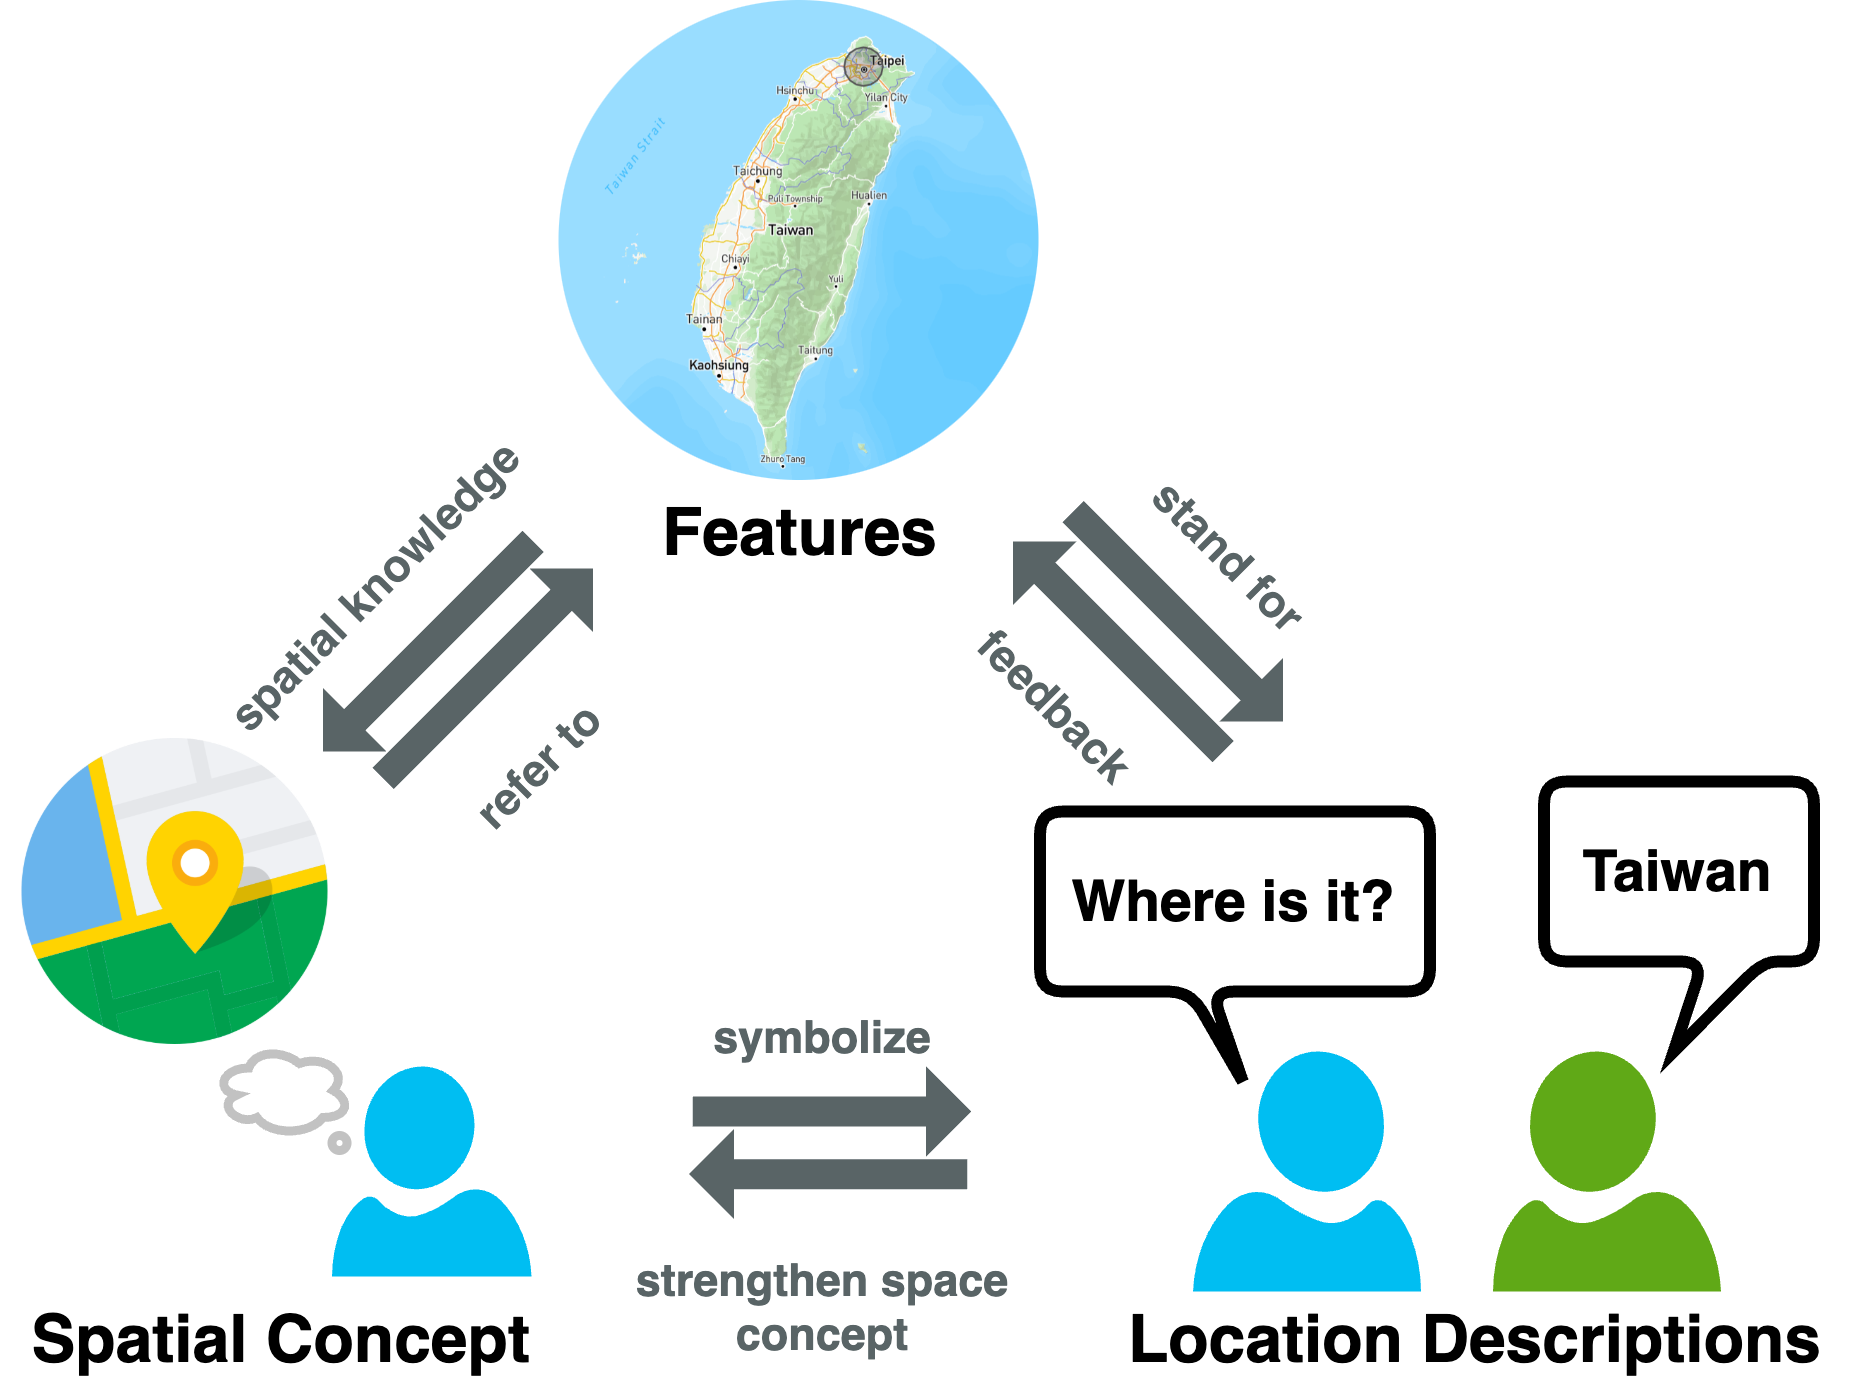
\includegraphics[width = \textwidth]{figures/congition.png}
\centering
\caption{位置描述語意三角形(改自\citet{RN128})}
\label{fig:congition}
\end{figure}

\section{知識本體與產生自然語言}

知識本體是一個形式化語言模型,具有以下三個核心要素:概念(concept)或類別(class)、實例(individual)與關係(relation),用以表示特定領域中物件的類型、結構、屬性、過程和關係\citep{RN24} 。地理現象可藉由知識本體形式化,舉例而言,行政區劃的空間關係「台北市包含大安區」這一現象,可以透過知識本體形式化為類別「County(縣市)」與「District(區)」,與之對應的實例為「台北市」與「大安區」,關係則可以表示為「hasContain(包含)」,即「台北市」作為一個實例,與「大安區」透過hasContain關係相連。這一語意結構的建模能力,使知識本體得以有效捕捉日常生活中的空間知識,並提供作為語意層次查詢與推理,例如,在該例中欲查詢行政區所包含的物件,即可獲得「大安區」的內容。

基於知識本體的語意建模能力,知識本體不僅可用於資料整合與邏輯推論,也逐漸被應用於產生自然語言的研究中。透過類別、實例與關係的結構化表示,可支持語言描述中角色、事件與語意關係的抽象建模,進而實現產生基於語意的文字。在非空間領域中,\citet{RN163}將知識本體應用在電子健康檔案上,將結構化紀錄的健康資訊轉換為自然語言文字,以協助醫療人員的解讀。在地理資訊領域中,經常以具備語意特徵的屬性資料作為地圖輔助描述\citep{RN165, RN166}。這類研究根據提出文檔計畫(document planning)過程中事先擬定好相關的參數及文字描述,使地理資料得以以自然語言描述方式呈現。惟這類研究多著重於地圖可視化中變量的敘述,如地形、設施數量等,較少涉及位置本身的語意建構與推論生成機制。

\section{知識本體與產生自然語言}

為了解決自然語言位置描述中所蘊含的語意模糊性與語境依賴性的挑戰,過往研究逐漸將語意層面納入從基於坐標之空間資料產生位置描述或逆向地理編碼中。此類研究大致可分為三類方法:依賴結構化地名資料(如地名辭典(gazetteers)和知識圖譜)和使用模糊邏輯與語意模型進行位置表示。

首先,地名辭典(gazetteers)作為逆向地理編碼的基礎資料來源之一,扮演結構化空間語意的角色,其常以地名、地點類型及其對應的空間足跡(spatial footprints)為三種基本構成元素\citep{RN122, RN159, RN31},試圖將語言中的地名對應到具體空間範圍及地理空間實體。近年來,為期獲得接近人類對於實體世界的表達,運用社群媒體資料建構更具有語意細緻度的地名辭典,藉此貼近人類對實體世界的描述習慣\citep{RN31}。相對於地名辭典的紀錄,\citet{RN23}則一樣透過社群媒體資料,但以地方圖譜(place graph)儲存人對實體世界的表達。該圖譜由空間物件及空間關係組成,因而產生合適地名不需要依賴傳統GIS空間分析方法,而是依照知識圖譜中記錄下自然語言式的空間關係三元組。儘管這些資料和儲存格式有助於提升逆向地理編碼產生位置描述的準確度和豐富度,結構化格式難以完整和全面涵蓋語言中隱含的模糊性與相對位置描述,在語意處理能力上仍具限制。

為克服此限制,研究開始探索以模糊邏輯與語意模型的方式來處理基於坐標之空間資料與位置描述的連結。例如,\citet{RN133}透過社群媒體資料計算隸屬函數(membership function)分析人類對「南/北加州」的認知,建立隸屬函數網格推估具有模糊邊界的地名空間範圍,有效捕捉地名的認知模糊性;\citet{RN164}針對相片地點的自然語言產生,提出一組顯著性指標(如照片地點是否常出現、地名的稀少和重要性、距離等),挑選適切之參考地名,再判斷其與目標坐標間的空間關係,並加上空間介詞來形成位置描述的方式。該研究針對地名產生僅能達到相對位置的描述,然而缺少在日常生活中也常使用到的絕對位置描述;而在\citet{RN128}的研究中,深入的討論了位置描述語意模糊性的原因,並以超值理論(supervaluation)為存在模糊的位置描述提出了一個定量的框架及機制,並透過問答系統使得研究貢獻得以應用於GIS上。該研究指出參考系統、空間物件(spatial object)和空間關係(spatial relationship)三者是造成模糊性的原因,首先,描述的參考系統影響了人類如何辨識空間物件及認知空間,存在於不同觀測者的空間認知和能力中,因此難以直接從描述中獲取。其次,空間物件可再細分為參考物與目標物件,不同觀測者間於認知中辨識出的物件也會有不同,除了物件的名稱外,物件的屬性資料也可能被用來進行描述,例如:大小和高度。最後,空間關係,例如「near」一詞根據不同觀測者會有其對應的定量值。該研究於過往對於空間認知的文獻設定變數改變其權重,以達成透過定性資料處理定量的地理資訊,並能提供都市導航的指路選擇。

整體而言,這些研究指出僅依賴坐標或結構化的地名資料儲存進行逆向地理編碼或語意查詢時,難以全面捕捉自然語言位置描述中蘊含的語意模糊性、情境依賴性與認知差異性。雖然透過給定語意建模或模糊邏輯等手段,有助於提升處理部分語意不確定性,卻仍缺乏一套能整合「位置描述詞彙、空間資料、語意空間關係、認知視角」的通用形式化表示與推理機制。此外,目前相關方法多偏重於語意輸出,但對於如何系統性建模空間語意概念之間的結構性關係,例如參考物、目標物與空間關係之間的角色與制約關係,尚缺乏深入處理。因此,本研究欲填補此一缺口,嘗試引入知識本體的形式化能力,結合語意規則推理,整合空間資料、語言表徵與空間認知概念,建構一套可推論之語意式位置描述的框架,進一步提升自然語言與空間資訊之間的語意連結與轉譯能力。


% !TeX root = ../main.tex

\chapter{研究方法}

本研究提出一個基於知識本體的語意位置描述三層式架構(ontology based semantic location description framework, O-SLD framework),旨在整合空間資料與自然語言中的位置描述語意,建構具有語意表達能力的位置描述之知識模型。圖 \ref{fig:framework} 顯示本研究架構,係結合知識本體、語意規則和圖資達成逆向地理編碼機制。透過本框架,期望為位置描述中的語意提供形式化模型,並強化空間資料、空間認知與自然語言之間的語意連結與互通性。在3.1節中,說明位置描述語意(O-SLD)三層式架構之設計,以達成空間資料、位置語意與位置詞彙的連結;在3.2節說明位置描述知識本體建構原則與內容架構;在3.3節描述規則設計準則及機制,以實現語意式位置描述的動態產生能力;在3.4節說明本研究評估方法,將採用SPICE(Semantic Propositional Image Caption Evaluation)作為評估指標。

\begin{figure}[!htbp]
\centering
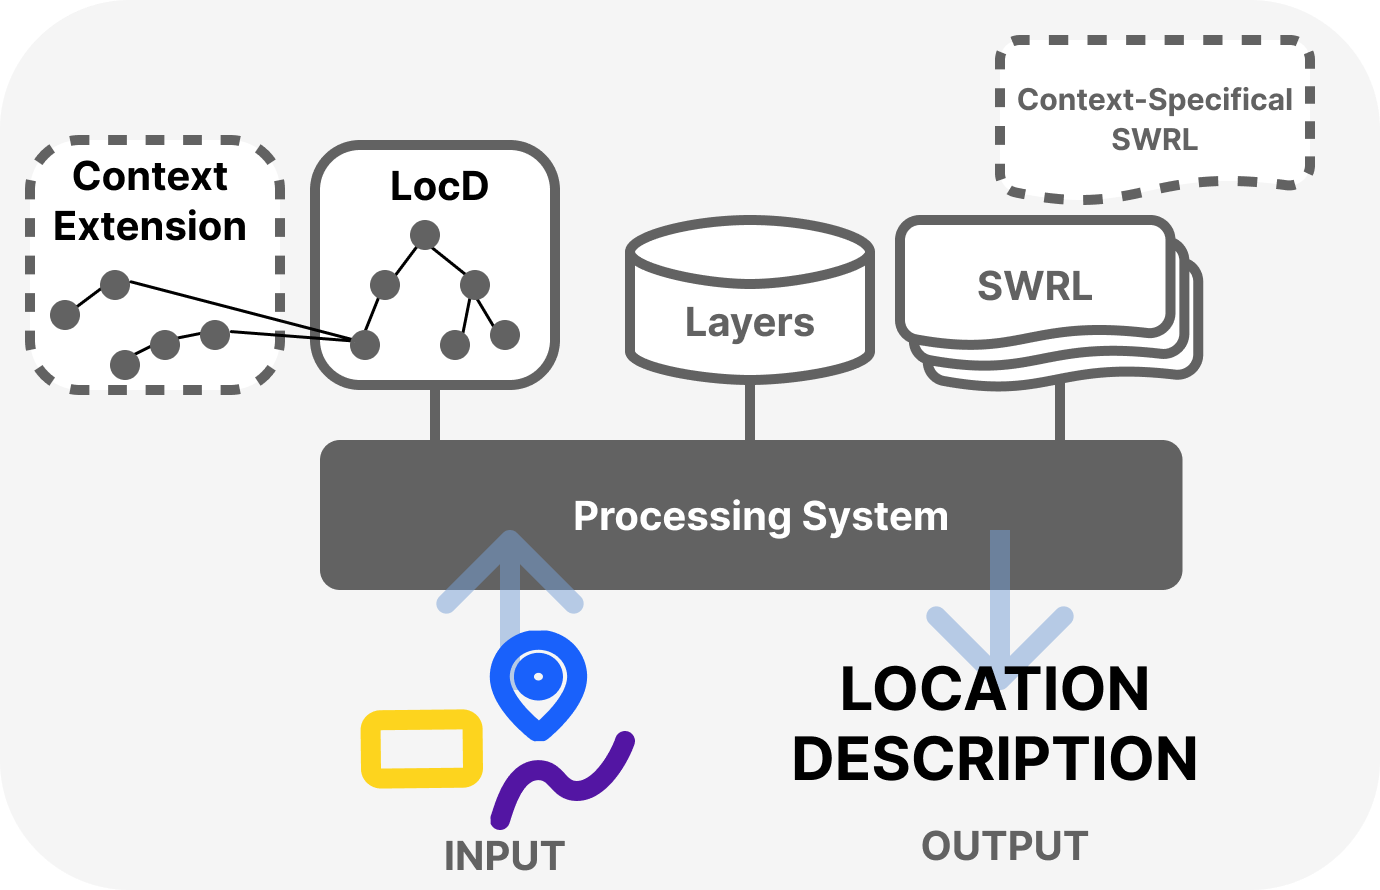
\includegraphics[width = 0.7\textwidth]{figures/research_framework.png}
\caption{研究架構圖}
\label{fig:framework}
\end{figure}

\section{位置描述語意(O-SLD)三層式架構設計}

為回應空間認知理論對人類位置理解的需求,並解決位置描述語意表徵上的挑戰,本研究設計了O-SLD三層式架構。該框架透過語意推理機制,能進一步從空間資料產生位置語意及語意式位置描述,能達成逆向地理編碼任務。框架的結構如 \ref{fig:three-layered} 所示,O-SLD三層式架構主要由三個層級組成:資料層、語意層和自然語言層。三層之間呈現自上而下的語意映射關係,分別對應空間資料、知識本體與語言表達,透過語意規則加以串連各層級,形成完整的語意推論機制。

\begin{figure}[!htbp]
\centering
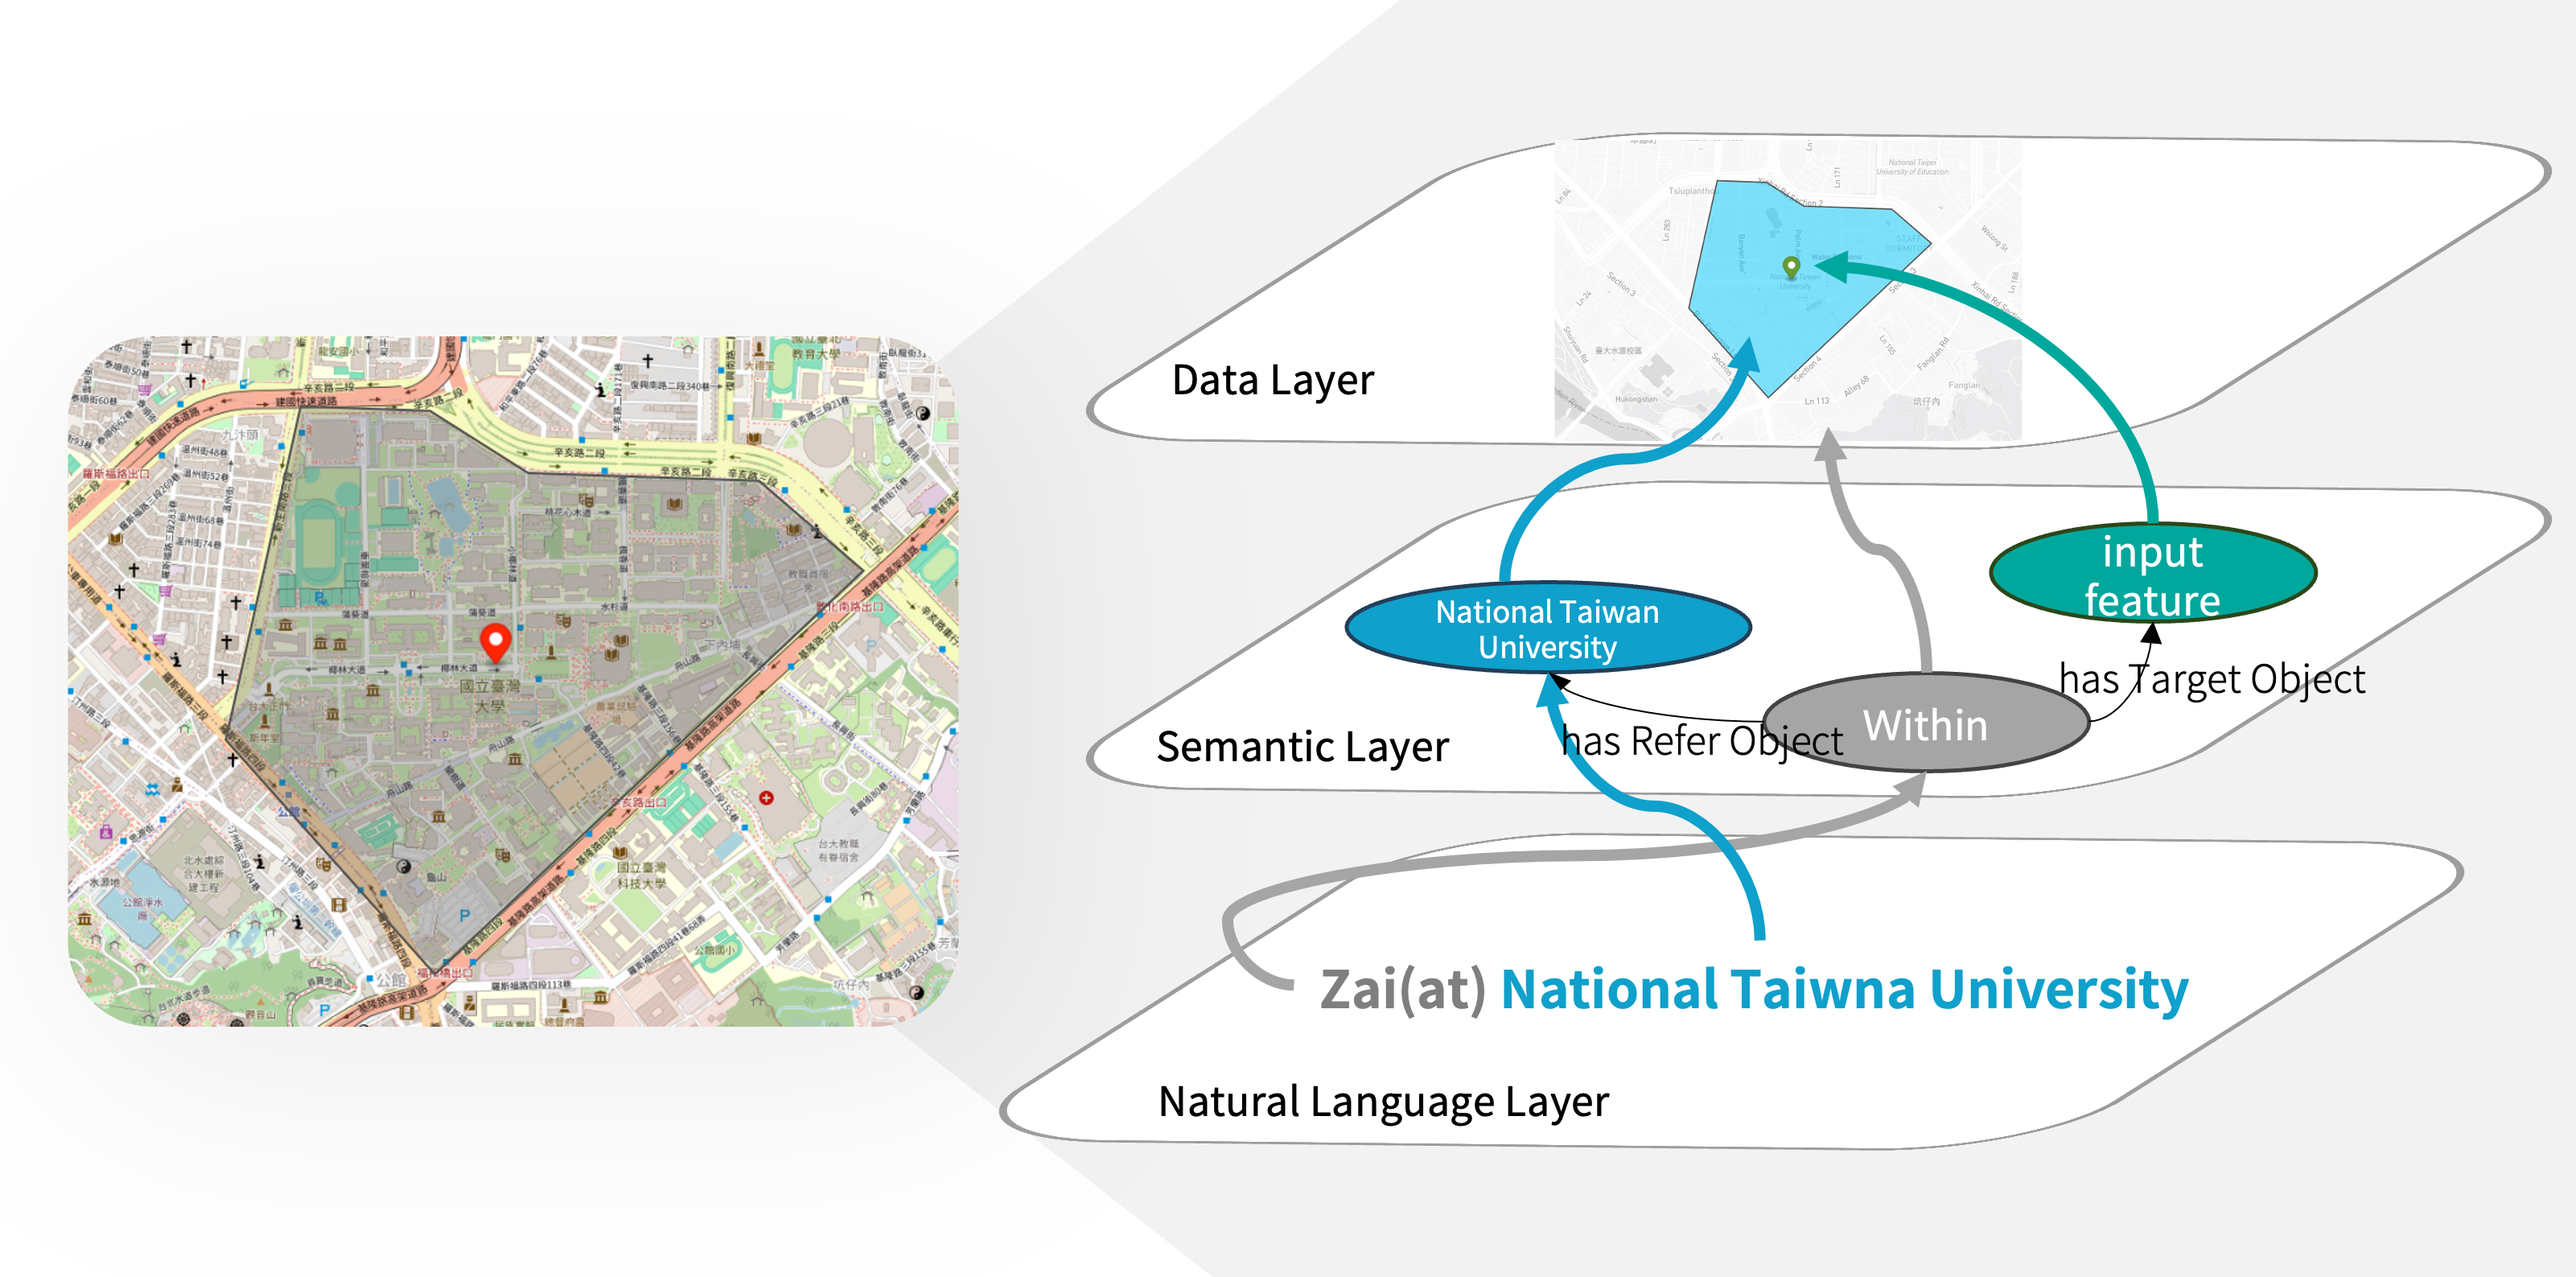
\includegraphics[width = \textwidth]{figures/three-layered.png}
\caption{位置描述語意三層式架構}
\label{fig:three-layered}
\end{figure}

「資料層」主要負責空間資料的紀錄與關係操作,包括點、線和面等的GIS Feature,以及其屬性與彼此間的空間關係。本研究將資料層獨立設計,旨在提供全面且詳盡的空間資料表示,支持進階的空間關係建模與語意推理。該層作為框架的基礎,為後續語意層與自然語言層提供圖資、詮釋資料及空間操作。

而「語意層」是框架的核心,負責知識本體的語意表徵與知識整合,透過知識本體存有形式化的特性,可整合來自GIS、空間認知和語言學等多領域的位置相關知識,支持位置語意的建構和語意位置描述的產生。本層的知識本體設計具有高可擴展性,能夠隨研究目標需求進一步擴充,從而豐富語意資訊。作為框架的中介層,語意層透過規則建構與推理機制,實踐各層級之間的互動,包含語意空間關係的推理及產生位置描述文字等。

最後,「自然語言層」負責將語意層中的知識與推理結果轉化為人類可讀之自然語言文本,並透過語言樣板與結構設定呈現自然語言式的位置描述給使用者。

本研究所提出之O-SLD三層式架構可應用於逆向地理編碼機制,能根據使用者輸入坐標位置,自動檢索並產生產生語意式位置描述。其核心功能在於:透過語意推理機制,將空間資料轉換為具有語意的知識表徵,進而轉譯成人類可理解之文字表達,從而促進使用者對位置之所在的理解與日常應用。以圖 2所示,當輸入點查詢位置描述時,機制參考各類參考物,並與之產生空間關係,詳細流程如下:首先,資料層到語意層的推論過程,判斷輸入圖徵與資料層中給定的各類參考物圖徵(如建物、行政區或地標等)之空間關係。若該點落在「台灣大學」這一圖徵內,則推論該點與「台灣大學」具有「位於(Within)」之空間關係,並將該資訊納入知識本體。接著,在語意層到自然語言層的過程,根據產生一組包含參考圖徵之語意及空間關係的知識本體,根據語料庫的規則進一步執行語意推論機制。最終,選擇情境下的語言樣板,產生對應到自然語言式之文字。例如,產生「在台灣大學」這一語意式位置描述。因此,結合O-SLD三層式架構可有效進行知識獲取與創造,進而轉換為文字式的位置描述。

\section{位置描述知識本體(location description ontology, LocD)}

本研究採用常見的知識本體建構過程METHONTOLOGY\citep{RN143},其建構過程包含需求規範、知識獲取、概念化、整合、實作與評估等七個階段,用以建立任務為導向的位置描述知識本體(LocD)。圖 \ref{fig:locd_framework} 所示為本研究發展之LocD知識本體之框架,係結合上層知識本體及橋接之知識本體,以達成位置描述中的語意表達。

本節首先說明所使用之上層知識本體,以提供在語意領域中整合基礎及互通能力,亦能有效降低語意重複與歧異產生。其次,說明位置描述知識本體中兩個子集結構:「圖徵及性質」和「位置描述與空間概念」。前者對應O-SLD三層式架構中的「資料層」,旨在定義空間資料如何介接知識本體,例如「台灣大學」作為Feature,存在幾何類型—「面」、名稱—「台灣大學」和類型—「大學」等資訊,這些資訊將分別記錄於「圖徵與性質」之子集中。同時,輸入圖徵與參考圖徵產生的空間操作(spatial operation)結果也將記錄於其下;後者則對應O-SLD三層式架構中的「自然語言層」,旨在定義位置描述語言中的空間介詞與方位詞,並賦予其對應之語意空間關係。這些語意元素分別記錄在「位置描述與空間概念」之子集中,進一步支持位置描述文字的語意。

\begin{figure}[!htbp]
\centering
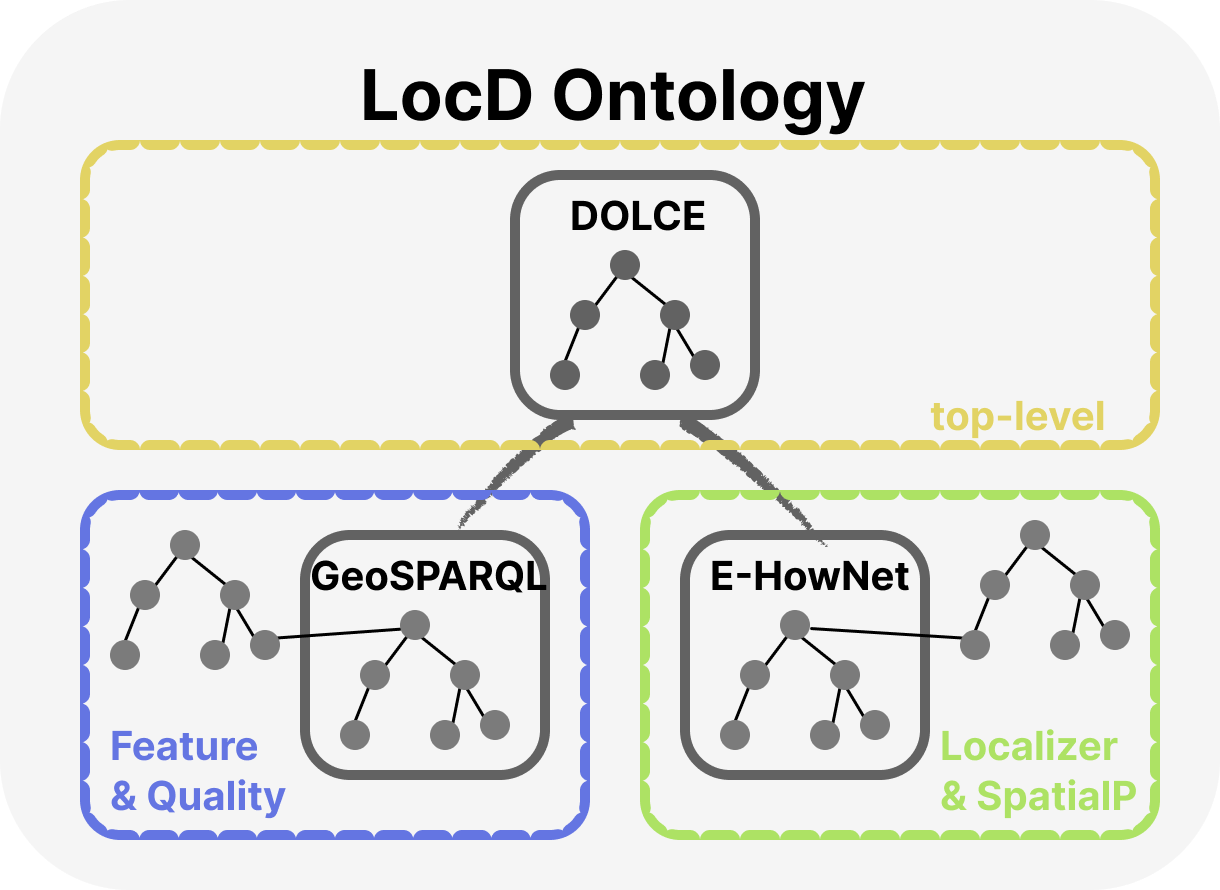
\includegraphics[width = 0.7\textwidth]{figures/Locd_framework.png}
\caption{位置描述知識本體框架}
\label{fig:locd_framework}
\end{figure}

\subsection{上層知識本體}

達成語意互通,本研究採用三個上層知識本體框架進行知識本體建構的整合既有知識(參見圖 \ref{fig:locd_top} ),分別為:Descriptive Ontology for Linguistic and Cognitive Engineering (DOLCE)、GeoSPARQL Ontology和廣義知網知識本體(Extended-HowNet Ontology, E-HowNet ontology)。位置描述的產生過程以空間認知的三個核心概念構成其基本結構,分別為Feature (\textit{dul:Feature})、空間概念(\textit{locd:SpatialConcept})及位置描述(\textit{locd:LocationDescription})。此外,形塑空間概念的組成元素則記錄於性質(\textit{dul:Quality})之下,使得知識本體可涵蓋空間認知過程形成位置描述的關鍵特徵,並有助於各個子類語意關係明確化。上層知識本體的引入,係基於該結構之考量,以下詳述個別內容:

\begin{figure}[!htbp]
\centering
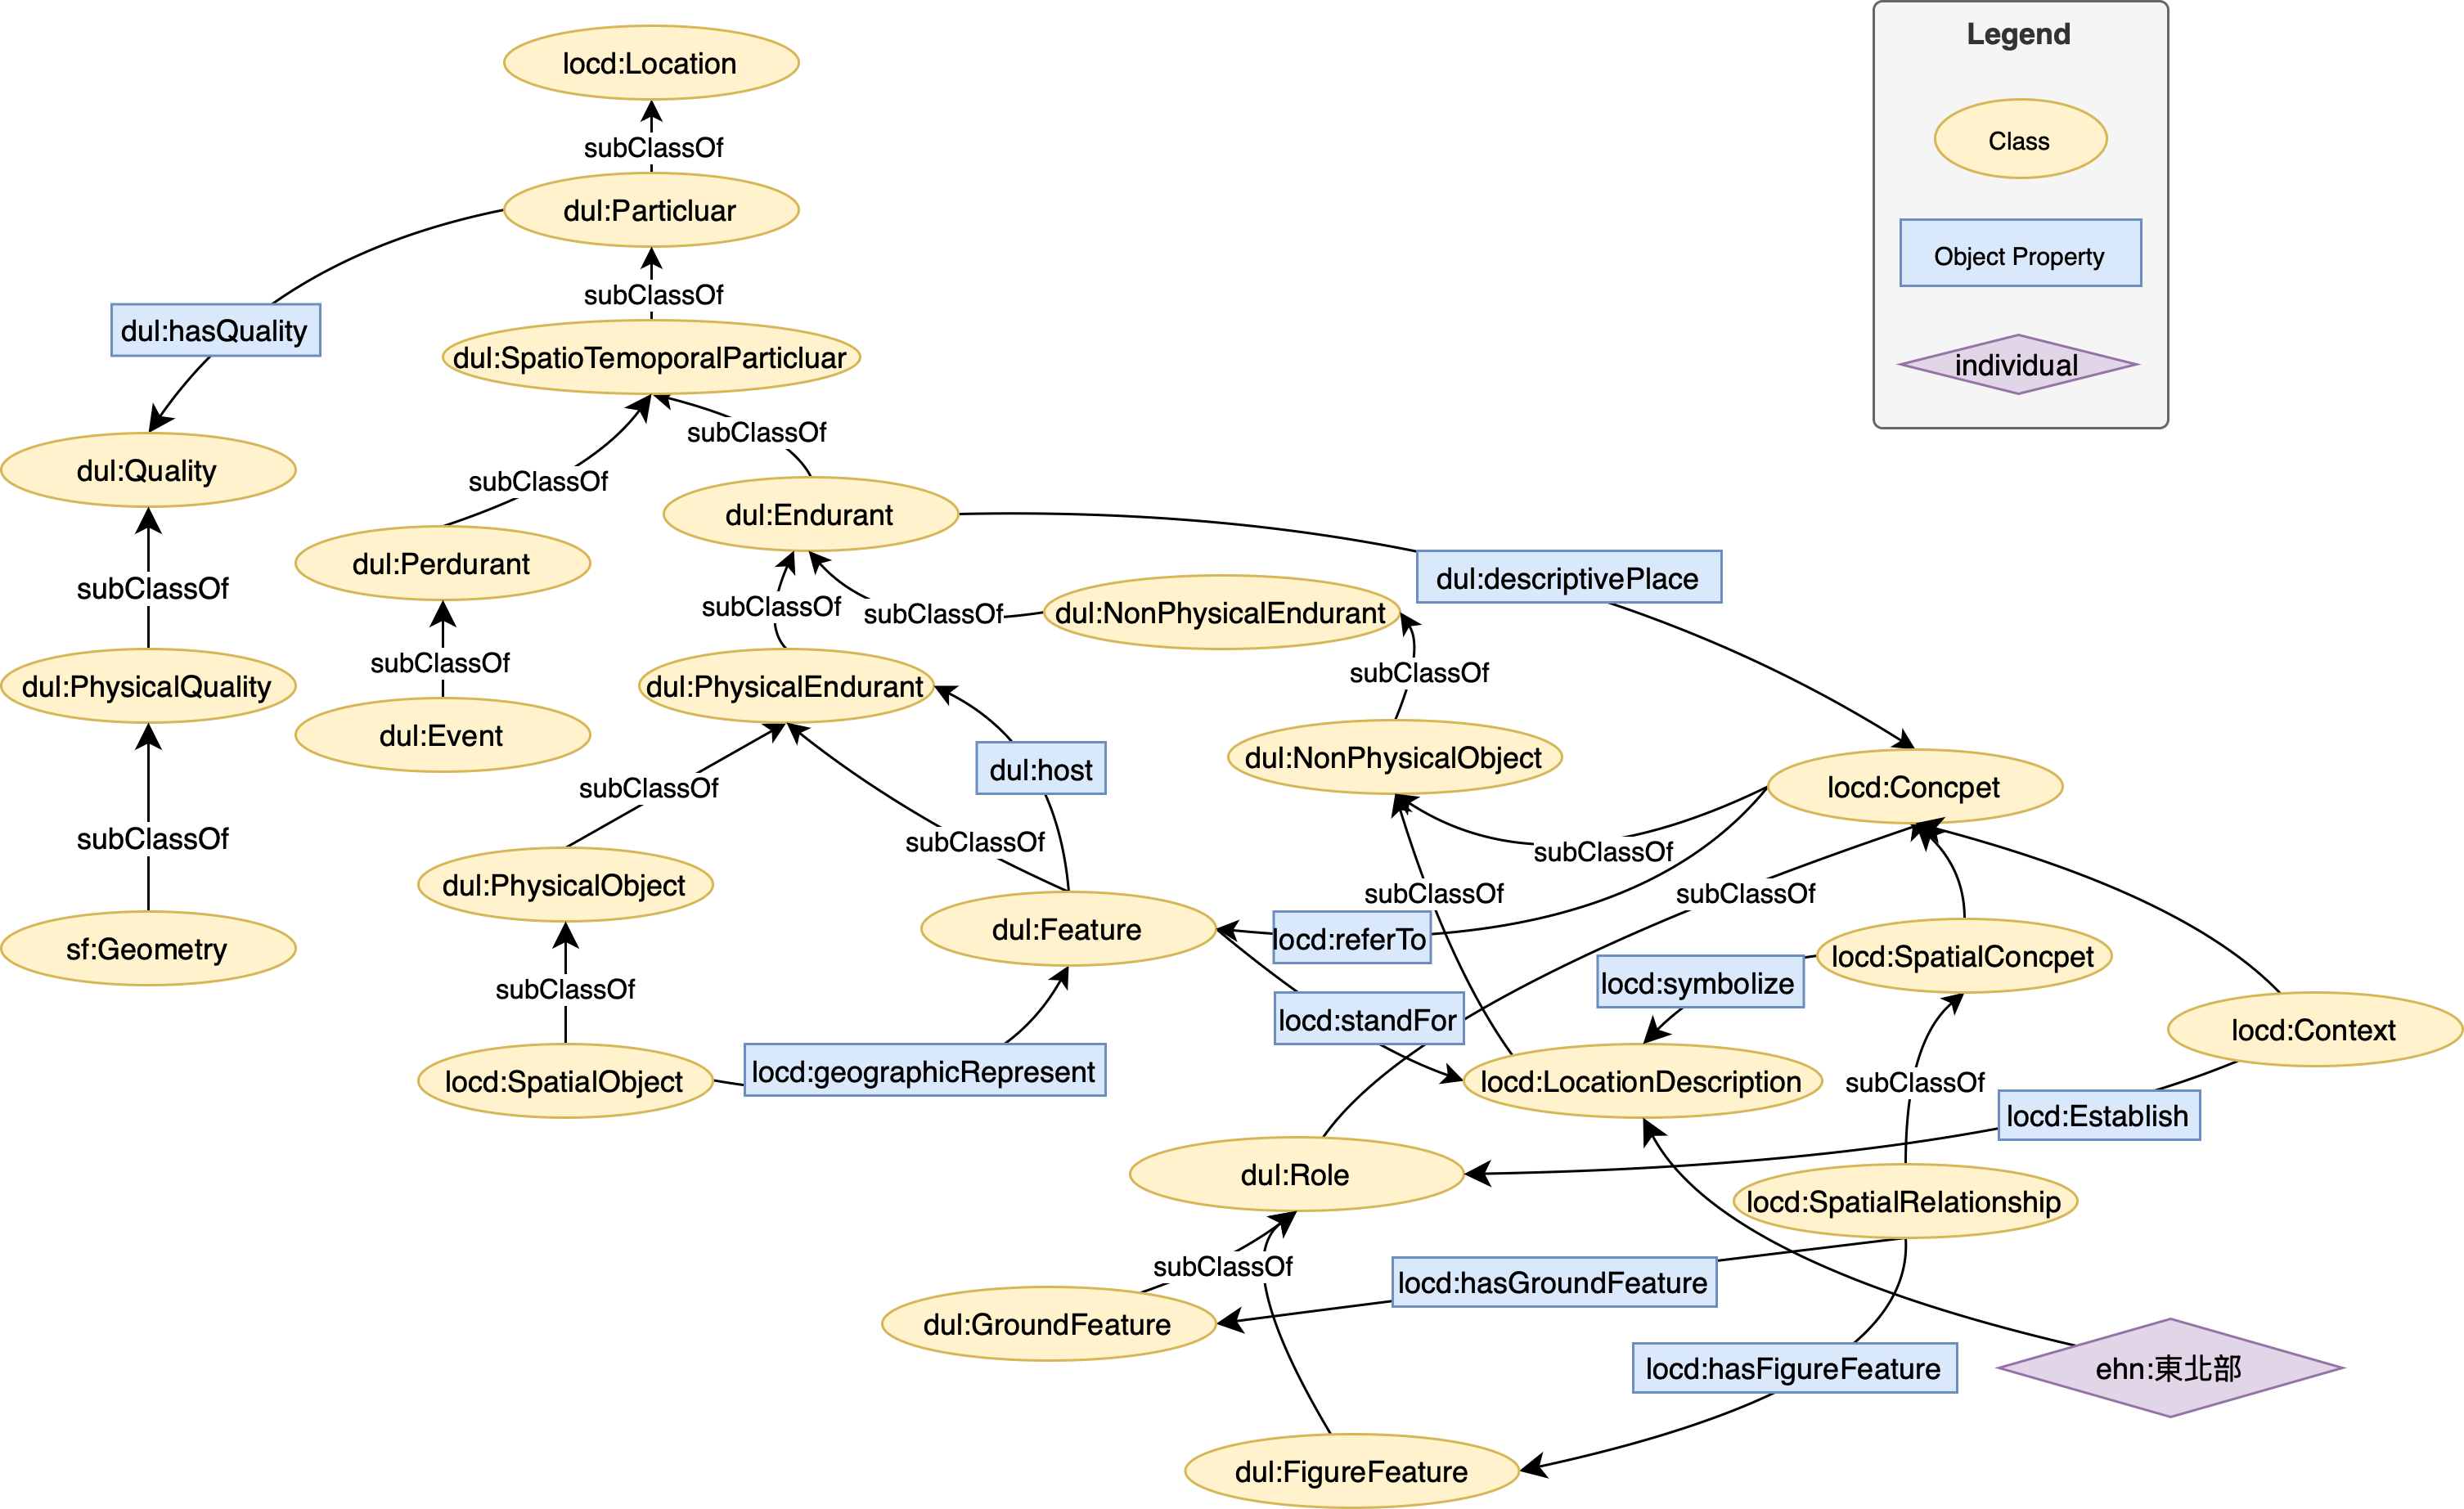
\includegraphics[width = \textwidth]{figures/LocD_top_level.png}
\caption{位置描述知識本體上層架構}
\label{fig:locd_top}
\end{figure}

\subsubsection{Descriptive Ontology for Linguistic and Cognitive Engineering (DOLCE)}

為建構具語意推理能力和整合不同領域的位置語意資訊的的位置描述知識本體,本研究採用經邏輯語言公理化(axiomatized)的上層知識本體 DOLCE作為語意架構基礎,其實體分類系統與性質描述機制可有效支持位置語意的建模與跨領域整合(參見圖 \ref{fig:dolce} )。

\begin{figure}[!htbp]
\centering
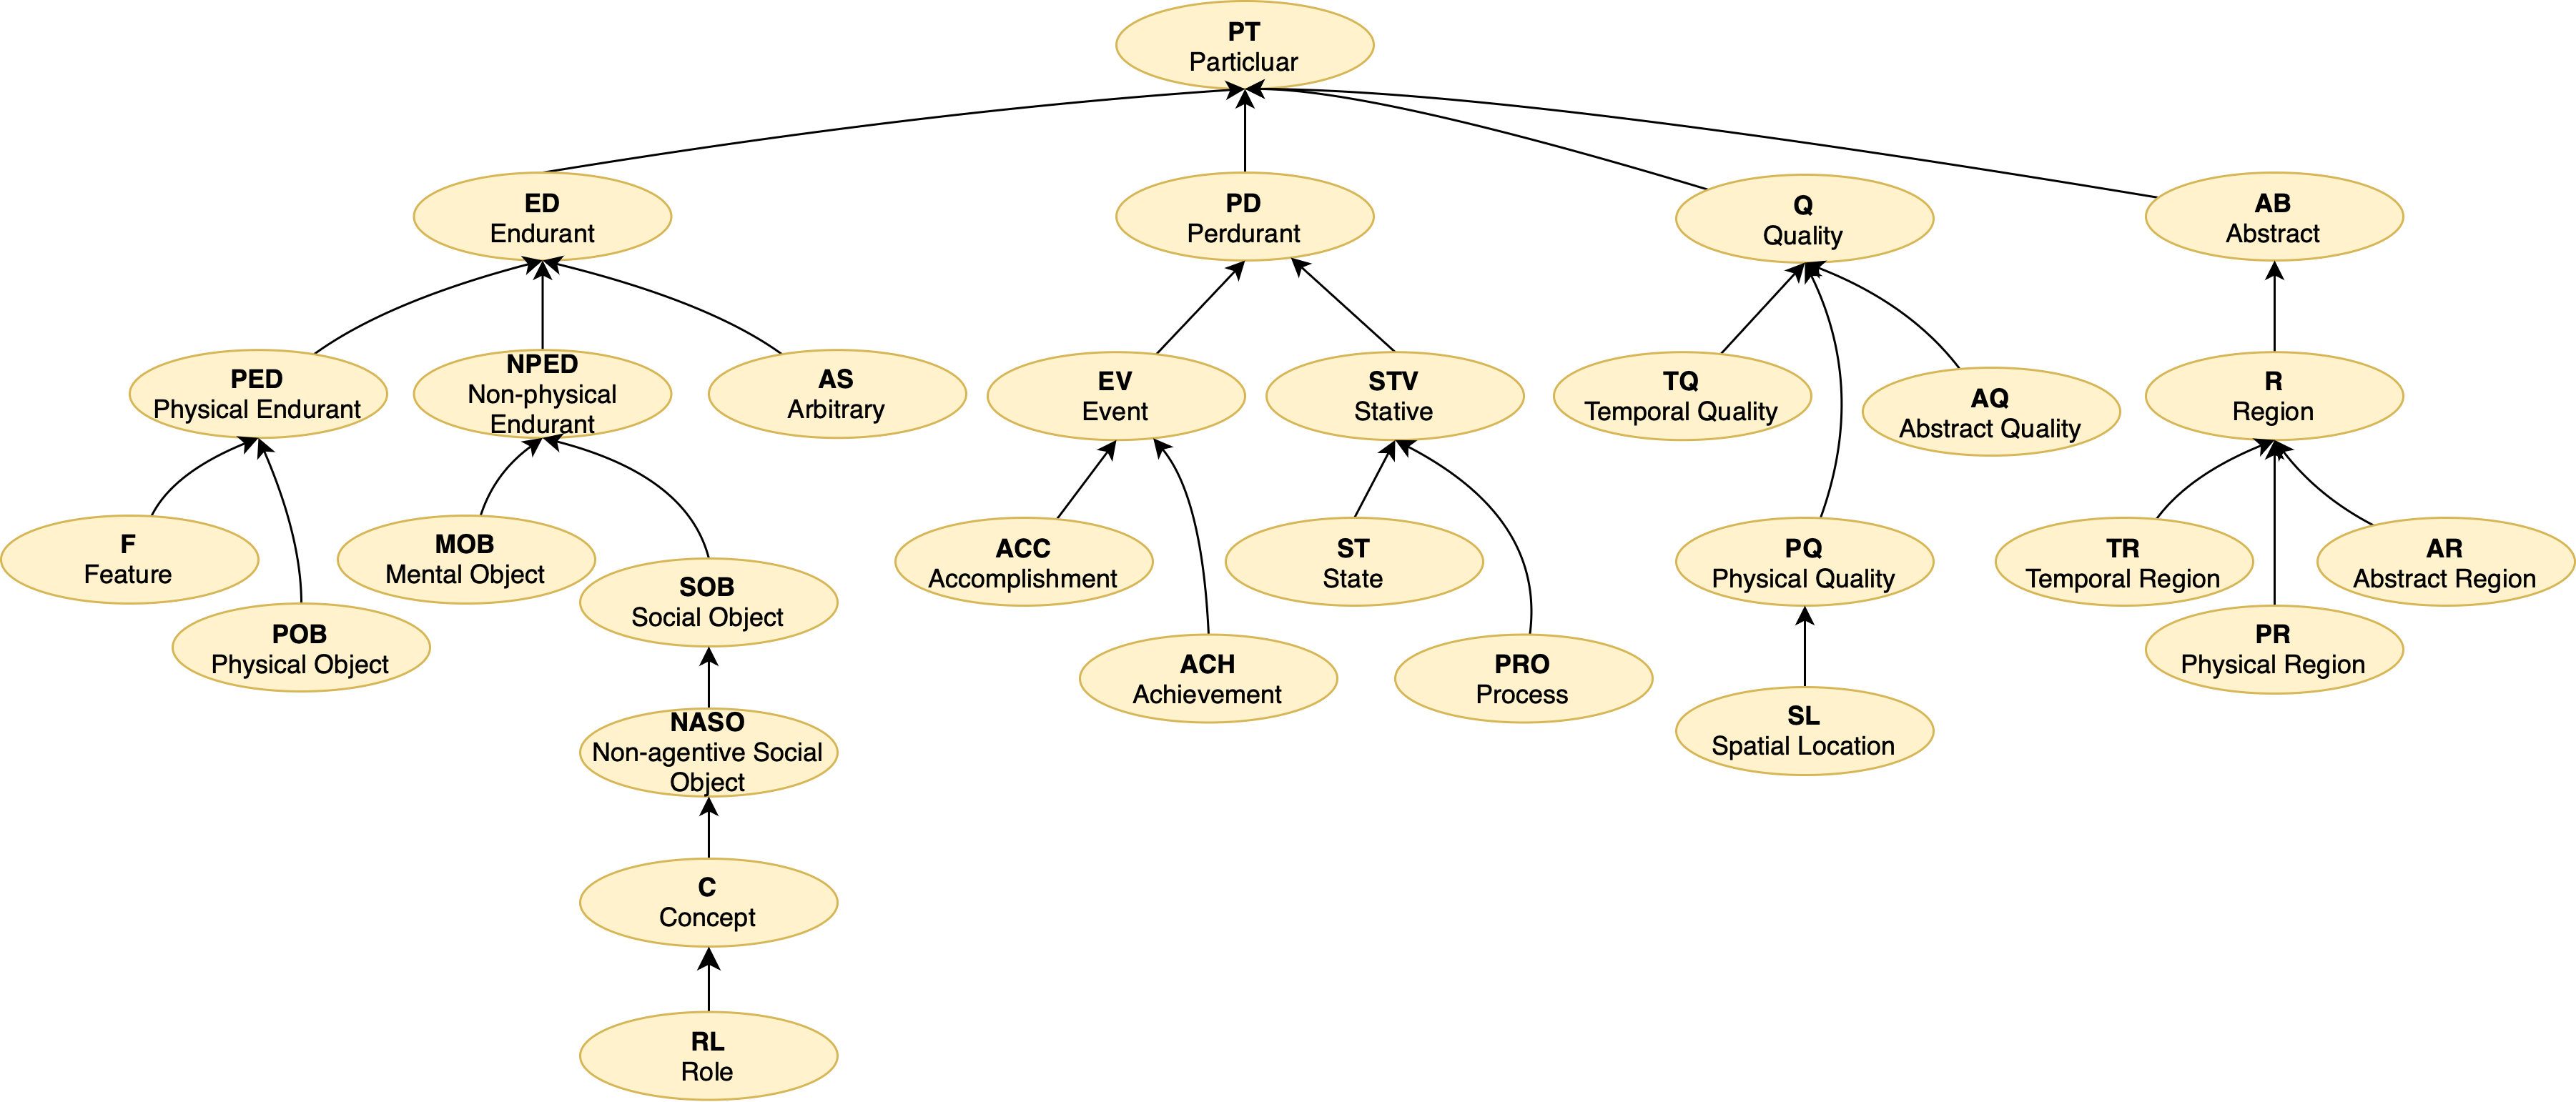
\includegraphics[width = \textwidth]{figures/dolce.png}
\caption{DOLCE的分類法}
\label{fig:dolce}
\end{figure}

DOLCE旨在基於認知和語言考量來建立一個人類日常所使用和理解的事物之常識模型作為一個基礎知識本體,核心目的是提供一般性的範疇和關係,以建構一個連貫的現實理解框架\citep{RN86}。同時,DOLCE已廣泛應用於社會技術系統、製造業、金融交易和文化遺產等領域,在地理資訊領域中,亦透過DOLCE建立跨領域術語與知識結構,支援不同領域間的語意中\citep{RN195, RN193}。

對應於人如何理解環境的過程,會存在物理的地理環境與抽象後的表徵(例如GIS上的Feature或文字式的位置描述),DOLCE的分類結構將實體第一階層區分為「Endurant(持續體)」和「Perdurant(發生體)」。Endurant指的是在任何存在的時間點,其所有部分都在,例如:一棟建築;反之Perdurant是部分臨時存在的,也就是在任何展開的時間點,只有一部分存在,例如:牆壁上的裂縫。

進一步地,第二層上Endurant又依其是否具備物理性質區分子類,分別為「Physical Endurant(物理持續體)」指的是具有具體的物理性質,和「Non-Physical Endurant(非物理持續體)」多指抽象的或社會性的實體,例如:「詞彙(word)」作為位置語意的語言表徵,屬於非物理持續體中的符號化實體;而「詞意(word sense)」作為語意,亦屬於非物理持續體中的抽象概念。在本研究發展之位置描述知識本體中,將Feature劃分為Physical Endurant,而其隱含的空間概念則是Non-Physical Endurant。以「台北101」為例,其可以是一個實際存在的物理空間特徵(為Physical Endurant),但在概念層次中則可能代表一個隱性的概念(為Non-Physical Endurant下的Concept),例如台灣的最高樓等。

此外,DOLCE 不僅關注於實體的分類,亦在Quality(性質)上提供完整的上層知識本體結構,使其能夠有效地描述可被感知與測量的東西與實體之間的依存關係,在本研究的任務中對應於Feature及其屬性資料,這一分類方法可應用於區分地理物件的測量屬性(如坐標值和樓高等)與其語意屬性(如類型、重要性和歷史文化價值等),進一步提升Feature的語意表達範疇。更詳細來說,性質被視為依附於特定實體的特徵,無法獨立存在。例如,「顏色」作為性質的一種,僅當它與某一物體(例如一棟建築)相關聯時,才具備語意價值。這種對於性質的描述,使得 DOLCE 能夠在語意推理中明確區分性質本身與其承載的實體。如同實體子類之區分,DOLCE將性質進一步區分為「Physical Quality(物理性質)」與「Abstract Quality(抽象性質)」,分別對應於具體可測量的屬性(如重量和長度等)與較抽象的特徵(如情緒和評價等)。

綜上所述,DOLCE 具備明確的分類體系與語意結構設計,能夠有效支援位置語意資訊的組織與推理。本研究將其作為核心上層知識本體,整合位置描述所需之Feature的語意、性質分類與空間概念,進一步推進跨領域語意理解與空間資料之結合,建立更具解釋性與可推理性的語意位置描述模型。

\subsubsection{GeoSPARQL Ontology}

為確保空間資料的可解釋性與可互操作性,本研究將 GeoSPARQL作為表達空間資料幾何特徵與空間操作的主要語意框架,並結合 DOLCE進一步提升位置語意推理的能力。

GeoSPARQL Ontology由開放地理空間協會(Open Geospatial Consortium, OGC)所制定的語意網標準,旨在表達空間資訊支援查詢與推理(參見圖 \ref{fig:geosparql} )。其定義了「Feature(圖徵)」、「Geometry(幾何)」等類別,前者代表特定論域中的離散的空間現象,不論其是否有明確邊界,其皆具有可識別性,例如:行政區界、山脈及颱風等;而後者為在空間中一組連貫的直接位置,這些位置存在於空間參考系統內,用來表達Feature的幾何表現(例如形狀、範圍或位置)。

\begin{figure}[!htbp]
\centering
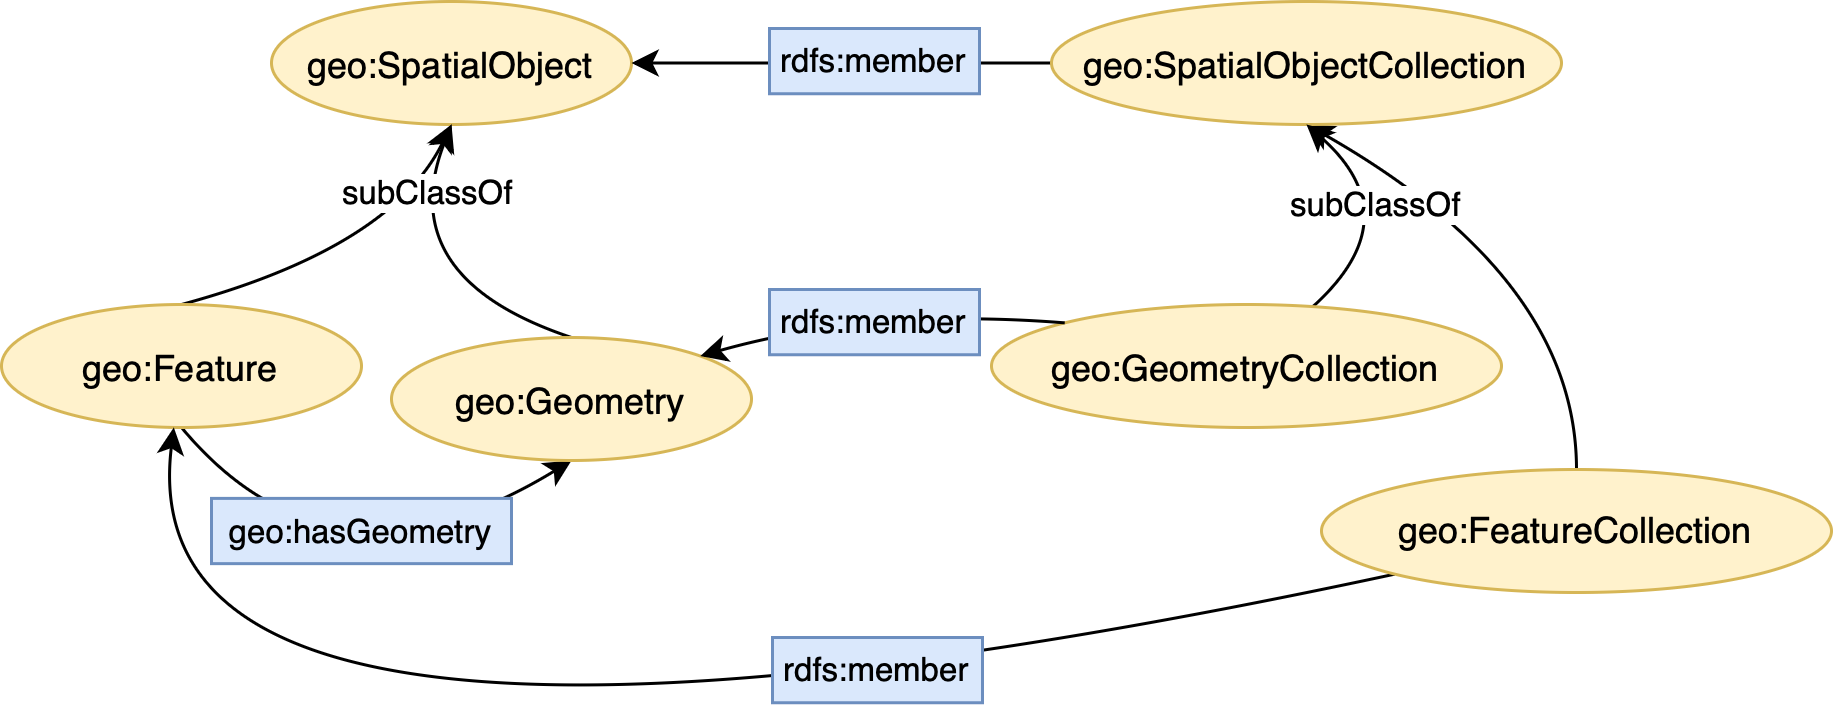
\includegraphics[width = 0.7\textwidth]{figures/geosparql.png}
\caption{GeoSPARQL Ontology的基礎類別及屬性}
\label{fig:geosparql}
\end{figure}

除了基本結構定義外,GeoSPARQL亦擴展了空間關係的描述能力,納入以DE-9IM (Dimensionally Extended Nine-Intersection Model)為基礎所建構的拓撲關係(topological relation),包含:「equals(相等)」、「disjoint(不相交)」、「intersects(相交)」、「touches(接觸)」、「within(內含於)」、「contains(包含)」、「overlaps(交疊)」和「crosses(橫越)」。

\subsubsection{Extended-HowNet Ontology (E-HowNet Ontology)}

為從語意產生文字,本研究選擇E-HowNet作為詞庫。E-HowNet為中央研究院資訊所詞庫小組開發,內容涵蓋九萬多詞條與知網連結,以簡單概念取代義原,具有較容易轉換為自然語言的特性\citep{RN186}。本研究鑒於詞彙表徵與表達式概念的特性,將其作為預定義好的詞意及詞彙對照關係,結合DOLCE對於概念與實體的分類,以達成位置描述中空間關係的語意表達。

以「上」該筆詞條為例(參見\ref{tab:ehownetDemo}),詞彙背後所代表的詞意(即E-HowNet表達式)係為「upper|上」,當中「upper」可對應到GIS中的空間關係操作結果,而係根據與特定參考物產生空間關係而達成。又以「縣界」該筆詞條為例,其空間關係係為「boundary」,而該筆詞條限制的參考物特徵為「county|縣」。

綜述而言,根據前述之上層知識本體和文獻蒐集建構本研究的位置描述知識本體,以形式化位置知識和貢獻於位置描述相關的概念使得空間資料得以與位置語意及位置描述文字連結,使GIS能納入對個人對於空間位置與地點的表達。\ref{tab:perfix}羅列了在本研究發展位置描述知識本體上使用到的既有知識本體的前綴(prefix)和網址。

\begin{table}[htbp]
\centering
\caption{E-Hownet之詞條範例:「上」及「縣界」}
\label{tab:ehownetDemo}
\begin{adjustbox}{max width=\textwidth}
\renewcommand{\arraystretch}{1.4}
\begin{tabular}{
>{\centering\arraybackslash}m{1.5cm} 
>{\centering\arraybackslash}m{2.5cm} 
>{\centering\arraybackslash}m{2.5cm} 
>{\centering\arraybackslash}m{1.5cm} 
>{\centering\arraybackslash}m{1.2cm} 
>{\centering\arraybackslash}m{1.8cm} 
>{\centering\arraybackslash}m{3.5cm} 
>{\centering\arraybackslash}m{3.5cm}
}
\toprule
node\_id & type & name & word & pos & pos\_long & meaning & ehownet \\
\toprule
w\_19813 & attachWord & 上.Ncd.1 & 上 & Ncd & Ncda & on, above & \{upper\textbar 上\} \\
\hline
w\_20079 & word & 縣界.Na.1 & 縣界 & Na & Nad & county boundary & \{boundary(\{county\textbar 縣\})\} \\
\toprule
\end{tabular}
\end{adjustbox}
\end{table}

\begin{table}[htbp]
\centering
\caption{既有知識本體之前綴與網址}
\label{tab:perfix}
\begin{adjustbox}{max width=\textwidth}
\renewcommand{\arraystretch}{1.4}
\begin{tabular}{>{\centering\arraybackslash}m{3cm} >{\arraybackslash}m{13cm}}
\toprule
前綴 & 網址 \\
\toprule
\texttt{dul} & \texttt{http://www.ontologydesignpatterns.org/ont/dul/DUL.owl\#} \\
\hline
\texttt{geo} & \texttt{http://www.opengis.net/ont/geosparql\#} \\
\hline
\texttt{ehn*} & - \\
\toprule
\multicolumn{2}{l}{\textit{Note:} *E-HowNet知識本體雖為知識本體之結構,然其並無發佈RDF/OWL格式,因而本研究以 ehn 作為代稱。} \\
\bottomrule
\end{tabular}
\end{adjustbox}
\end{table}

\subsection{圖徵及性質}

在GIS中,空間物件會被抽象化為Feature及其屬性,即一空間物件會存在兩個實體類別\textit{dul:Feature}和\textit{dul:Quality},本小節將詳細介紹圖徵及其屬性的定義與範疇。

為實現位置描述,區分目標物及參考物至關重要,例如:對於「台灣大學位於羅斯福路上」這一位置描述而言,涉及到的Feature包含「台灣大學」作為目標物,以及「羅斯福路」作為參考物。因此,位置描述中的目標物(\textit{locd:FigureFeature})和參考物(\textit{locd:GroundFeature})設計為角色(\textit{dul:Role})的子類,以明確定義兩者在知識本體中作為角色的語意,即當特定條件或時間下實體會被視為特定角色,可有效區分\textit{dul:Feature}作為GIS中圖徵存在與在位置描述中的目標物和參考物的存在區別。

此外,在DOLCE中\textit{dul:hasQuality}被設計用來描述\textit{dul:Endurant}和\textit{dul:Quality}的關係,即Endurant擁有某種性質。作為\textit{dul:Endurant}的子類,前述定義之\textit{dul:Feature}、\textit{locd:FigureFeature}和\textit{locd:GroundFeature}亦繼承了其物件屬性\textit{dul:hasQuality},因此目標物和參考物也同樣擁有性質(\textit{dul:Quality}),以此記錄下Feature所擁有的語意特徵,例如,建物有高度和外觀等性質、地標有重要性和文化價值等性質。

同時,性質可進一步區分為物理性質(\textit{dul:PhysicalQuality})及抽象性質(\textit{dul:AbstractQuality})。其中,非物理性持續體僅能擁有抽象性質,而物理性持續體不在此限,除物理性質外,亦可擁有抽象性質。例如:「台北101」作為一個物理存在的建築物,除了高度、位置等物理屬性,亦可具有地標、社經中心等抽象性質。

為增加性質的語意描述能力,本研究引用\citet{RN39}提出的地方面向(place facet)架構,以此為基礎發展知識本體中的\textit{dul:Quality}子類。地方面向係指地方的類型資訊,用以探討地方這一模糊概念的具體形式化結構。在本研究中,將四個子類置於性質底下,並以物理與非物理作為區分。舉例而言,人類中心面向(\textit{dul:AnthropocentricFacet})、衍生性面向(d\textit{ul:DerivedFacet})和語言面向(\textit{dul:LinguisticFacet})為抽象性質(\textit{dul:AbstractQuality})的子類,而具有具體的空間及物理屬性的地理面向(\textit{dul:GeographicFacet})則為物理性質(\textit{dul:PhysicalQuality})的子類,以作為\textit{dul:Quality}的細化分類,以強化對Feature在其屬性資料上的語意表達(參見圖 \ref{fig:locd_quality} )。

\begin{figure}[!htbp]
\centering
\includegraphics[width = \textwidth]{figures/LocD_quality.png}
\caption{位置描述知識本體子集:圖徵與性質}
\label{fig:locd_quality}
\end{figure}

更詳細來說,第一階層為原始面向(primitive facets)、衍生性面向(derived facet)和語言面向(linguistic facet),衍生性面向是由不同原始面向的組合中產生。例如,衍生性面相中的子類類型(typology)與個人或社會提供的目的和目標直接相關,情感、功能、物理和空間等多個原始面向共同構成了對一個地方作為特定類型的描述。

在第二階層中,原始面向可細分為人類中心面向(anthropocentric facets)及地理面向(geographic facets)。前者關注個體或群體與地方之間的各種關係,強調地方與人的互動、感受和功能性,後者則描述地方的空間和物理屬性。進一步在第三階層的劃分,人類中心面向可細分成功能性及情感性兩子類,功能性依據個體與地方行為區分,包含:可供性(affordance)、活動(activity)、行動(action)和功能(function)等,而情感性中依照人的情感依戀及感受區分,包含:地方感(sense of place)、依戀(attachment)和顯著性(Prominence)等。另一方面,在地理面向可細分物理及空間兩子類,物理面向包含:部分、形狀、樣態和結構等,在空間面向包含:空間尺度(scale)、位置和幾何等。同時,衍生性面向除類型外,包含意義、認同(identity)和目的(purpose)等。

最後,有別於前述地方本身的特性,語言面向係為地方的指稱,使人們能夠溝通和分享關於地方的知識,為表達情感意義或談論地方的功能和物理特徵的渠道,其子類包含:地名(toponyms)、口語指稱(verbal reference)和本研究關注的位置描述。

表 \ref{tab:quality} 列出關於圖徵與性質之分類與應用,整理了相關類別、定義及範例,詳細解釋如下:表中的「類別」欄位對應知識本體中的「類別」,「類型」則分為圖徵與性質兩大類,並且包含每個類別的定義、說明及範例。以第一欄為例,\textit{locd:FigureFeature}表示在知識本體中存在該類別,並且位於「Feature」類別下,定義為「圖圖徵」,指的是圖徵中的定位物或目標物件,例如:「台灣大學位於羅斯福路上」中的「台灣大學」即為一個\textit{locd:FigureFeature}的實例。

\begin{table}[htbp]
\centering
\caption{圖徵與性質的類別、定義及範例}
\label{tab:quality}
\begin{adjustbox}{max width=\textwidth}
\renewcommand{\arraystretch}{1.4}
\begin{tabular}{>{\centering\arraybackslash}m{3.5cm} >{\centering\arraybackslash}m{1.5cm} >{\centering\arraybackslash}m{2cm} >{\centering\arraybackslash}m{10cm}}
\toprule
Ontology Class & 類型 & 定義 & 說明及範例 \\
\toprule
\textit{locd:FigureFeature} & 圖徵 & 圖圖徵 & 圖徵中的定位物或目標物件,例如:「台灣大學位於羅斯福路上」中的「台灣大學」 \\
\hline
\textit{locd:GroundFeature} & 圖徵 & 地真圖徵 & 圖徵中的參考物,例如:「台灣大學位於羅斯福路上」中的「羅斯福路」 \\
\hline
\textit{locd:Prominence} & 性質 & 顯著性 & 能夠連結人類情感的程度,也包含物理面向,例如:「台北101」為台灣最高建築和強烈的都市意象 \\
\hline
\textit{locd:SpatialValue} & 性質 & 空間價值 & 能夠連結人類情感的程度,也包含物理面向,例如:「台北101」為台灣最高建築和強烈的都市意象 \\
\hline
\textit{locd:Specificity} & 性質 & 特殊性 & 地點對於人們的總體價值,例如:「信義區」為台灣重要的商業中心 \\
\hline
\textit{locd:Behavior} & 性質 & 行為 & 地點實際的物理性行為,例如:「大安森林公園」中閒晃 \\
\hline
\textit{locd:Action} & 性質 & 行動 & 地點可執行的意圖性活動,例如:「大安森林公園」中散步 \\
\hline
\textit{locd:Affordance} & 性質 & 可供性 & 地點可能提供的潛在活動,例如:「大安森林公園」提供邊哭邊跨年 \\
\hline
\textit{locd:Purpose} & 性質 & 目的 & 由情感、功能、物理、空間層面混合提供某個群體目的,例如:「國道」係為聯絡兩省(市)以上及重要交通設施或政經中心 \\
\hline
\textit{locd:Identity} & 性質 & 身份 & 地點對於某個群體共享的身份,例如:「人行道」對於行人來說可以是行人空間,而對於「開車族」而言可能是方便違停的地點 \\
\hline
\textit{locd:Typology} & 性質 & 類型 & 區分各種地方的方式,這些類型具有特定的情感、功能、物理和空間層面,例如:「道路」的目的係為提供交通流通的功能,同時也存在著空間範圍等不同面向 \\
\hline
\textit{locd:Address} & 性質 & 地址 & 以門牌定址作為空間參考系統的位置描述,例如:「台灣大學」為台北市大安區羅斯福路四段1號 \\
\hline
\textit{locd:Locatum} & 性質 & 定位物 & 以空間關係作為參考系統的位置描述中的描述對象,例如:「台灣大學位於羅斯福路上」的「台灣大學」 \\
\hline
\textit{locd:SpatialRelationship} & 性質 & (語意上的)空間關係 & 以空間關係作為參考系統的位置描述,例如:「台灣大學位於羅斯福路上」的「位於…上」這一概念 \\
\hline
\textit{locd:Relatum} & 性質 & 參考物 & 以空間關係作為參考系統的位置描述中的參考對象,例如:「台灣大學位於羅斯福路上」的「羅斯福路」 \\
\hline
\textit{locd:Toponym} & 性質 & 地名 & 對地點的直接參照,例如:「台北」、台北的「公館」 \\
\hline
\textit{locd:PlaceDescription} & 性質 & 地方描述 & 用語言對於地點詳細描述的內容,例如:「大安森林公園是充滿綠樹的公園」 \\
\hline
\textit{locd:PartsandStructure} & 性質 & 部分和結構 & 地點的內部組成,例如:「國道」有「匝道」 \\
\hline
\textit{locd:FormandStyle} & 性質 & 形式和風格 & 地點的視覺化內容,例如:「道路」有高架、平面和地下之分 \\
\hline
\textit{locd:Scale} & 性質 & 空間規模 & 地點在不同層次或細節水平上的存在和意義,例如:「國界縣」在OSM的縮放層級為4 \\
\hline
\textit{locd:Geometry} & 性質 & 幾何 & 空間物件的幾何類型,例如:Feature的基礎幾何類型為點、線和面 \\
\bottomrule
\end{tabular}
\end{adjustbox}
\end{table}

\subsubsection{類型}

% 在前述衍生性面向中,類型(\textit{dul:Typology})作為其重要子類之一,涉及地方如何被人類歸類和識別,在位置描述產生過程中至關重要。為了系統性地描述不同類型的地方,本研究結合內政部頒布之《地形資料分類架構》的分類法(參見\ref{tab:topoItemDemo}),將其分類結構完整納入類型的子類。

該分類架構係參酌地形圖製圖傳統及經驗、考量基本地形圖應涵蓋之地形資料內容等因素,內容分類採樹狀階層結構,涵蓋粗略主題之上階層到特定主題的下階層,包含測量控制點、界線、人工構造物、交通系統和水系等十類。該分類編碼表提供詳盡的階層式分類及說明,可作為空間物件的類型語意資料。舉例而言,「9210100國界線」係為「兩國之間的界線經確定者,為國家領土歸屬之明確界線,常由國與國之間協定,依天然地形或地理位置而定之」。透過此類具明確語意的分類之結構,可有效支持圖徵個體在知識本體中之類型建模,並促進與其他地方面向(如功能、型態或社會角色等)的整合推理,例如,社會角色重要之物件視為「地標」類型,這樣的類型可提供作為參考物在位置描述上的重要程度語意資訊及位置描述語言組成結構中的元素。

\begin{table}[htbp]
\centering
\caption{地形資料分類編碼表}
\label{tab:topoItemDemo}
\begin{adjustbox}{max width=\textwidth}
\renewcommand{\arraystretch}{1.4}
\begin{tabular}{
>{\centering\arraybackslash}m{1.2cm} 
>{\centering\arraybackslash}m{1.2cm} 
>{\centering\arraybackslash}m{1.2cm} 
>{\centering\arraybackslash}m{2.5cm} 
>{\centering\arraybackslash}m{4cm} 
>{\centering\arraybackslash}m{5.5cm}
}
\toprule
中類 & 小類 & 細類 & 分類編碼 & 中文名稱 & 英文名稱 \\
\toprule
2 &  &    & 9200000 & 界線 & boundary line \\
\hline
  & 1 & 00 & 9210000 & 國界 & international boundary \\
  \hline
  & 1 & 01 & 9210100 & 國界線 & determined international boundary \\
  \hline
  & 2 & 00 & 9220000 & 省(市)界 & provinces/municipalities boundary \\
  \hline
3 &  &    & 9300000 & 人工構造物 & artificial structure \\
\hline
  & 1 & 00 & 9310000 & 房屋 & building \\
\bottomrule
\end{tabular}
\end{adjustbox}
\end{table}

\subsubsection{GIS空間操作}

在GIS中,空間操作(\textit{locd:SpatialOperatio})是處理和分析空間資料的關鍵技術。其中,拓樸(topology)、距離(distance)和方位(direction)關係是描述Features間的常見概念和分類(參見圖 \ref{fig:locd_spatialoperation} ),本小節將詳細介紹這三類空間操作的定義與範疇。

\begin{figure}[!htbp]
\centering
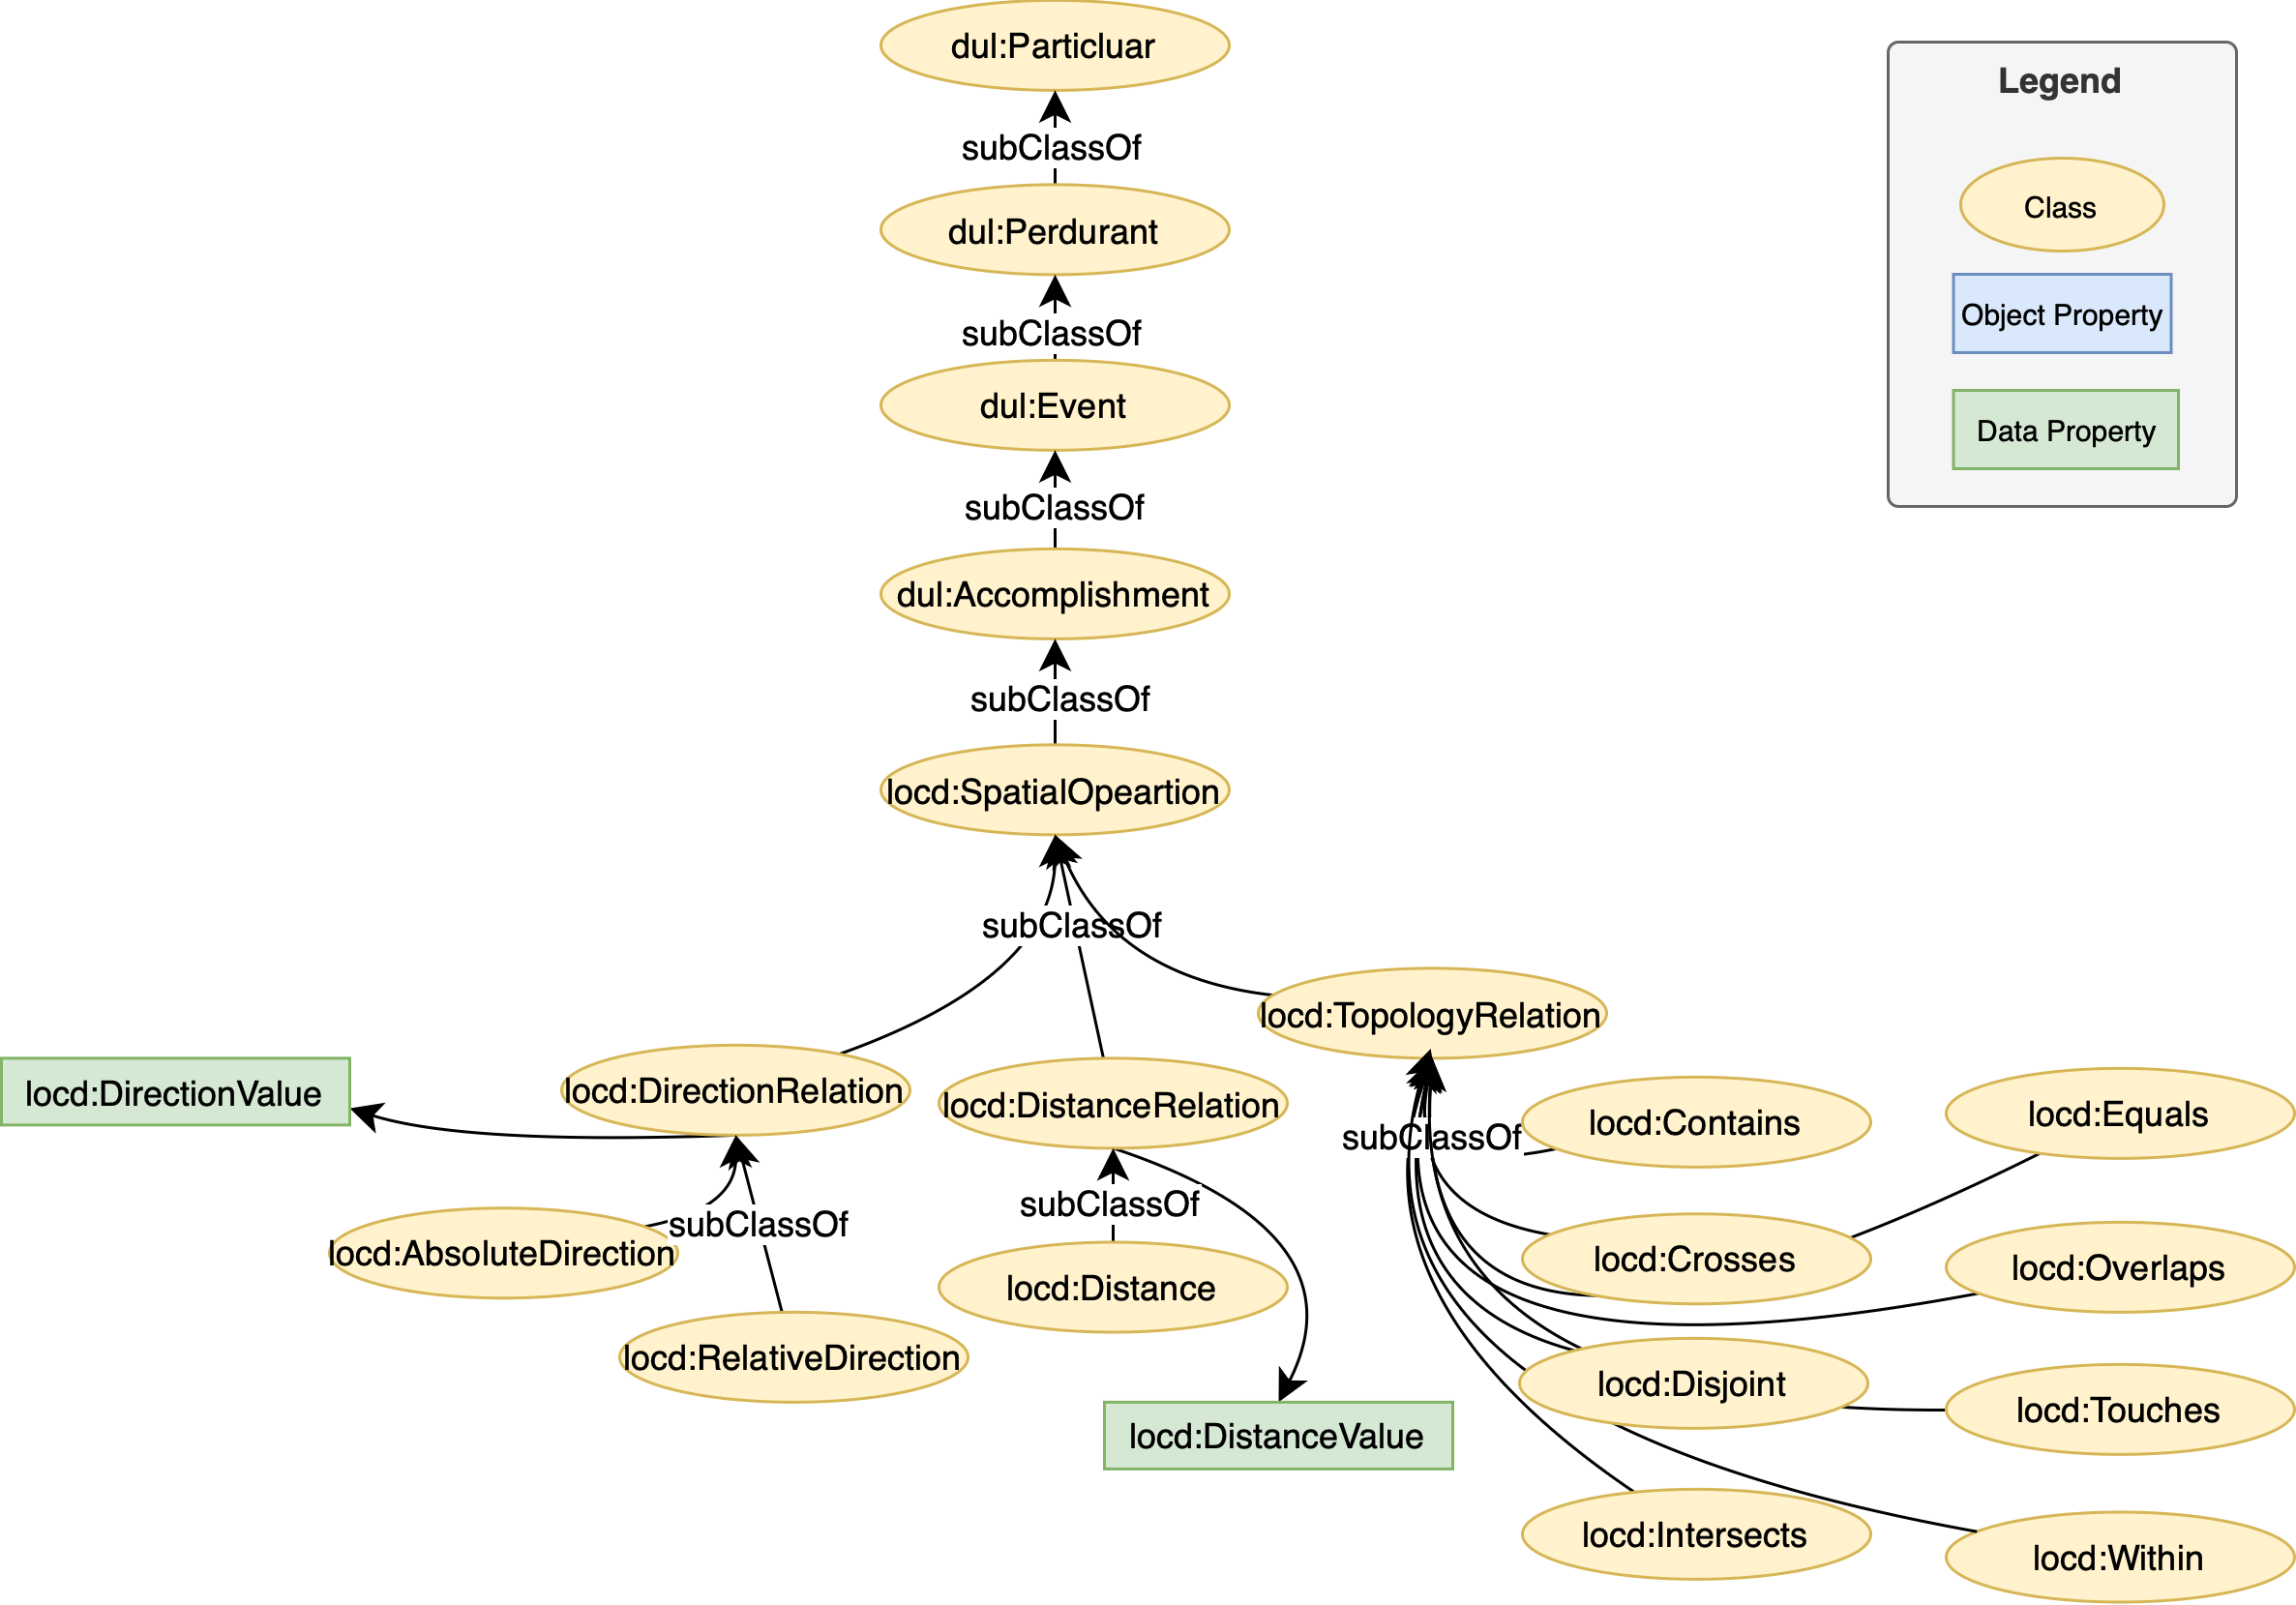
\includegraphics[width = \textwidth]{figures/LocD_spatialoperation.png}
\caption{位置描述知識本體子集:空間操作}
\label{fig:locd_spatialoperation}
\end{figure}

第一,拓樸關係係描述空間物件之間的相對的定性特性,包含相交、重疊和包含等特性。常見的拓樸關係透過維度延伸九交集模型(Dimensionally Extended Nine-Intersection Model, DE-9IM)形式化表示之,並廣泛應用在GIS的空間查詢與分析。第二,方位關係描述物件置於其他物件的相對方向,通常以方位角或羅盤方位來表達。常見的方位關係描述途徑有以下:方位矩陣模型(Direction Relation Matrix, DRM)透過矩陣方式表示物件之間的相對方向,如左、右、上、下\citep{RN183};基於象限的方向模型,將空間劃分為四象限(即東北、西北、東南、西南)或八方位(即北、東北、東、東南、南、西南、西、西北)來描述物件間的方向關係;角度計算則是使用數學方式計算兩點之間的方位角,適用於路徑分析與導航應用。第三,距離關係用於衡量空間物件之間的相對位置,以數值方式描述它們的接近程度。

\subsection{位置描述與空間概念}

在位置描述中,詞彙與概念性的詞意(即E-HowNet表達式)是區分語言表徵與概念的關鍵因素。此外在位置描述的結構上,主要包含地名、空間介詞與方位詞三元結構,本節說明如何結合E-HowNet的詞條與其在位置描述知識本體中的對應關係,並依照三元結構區分。

本研究發展之位置描述知識本體中(參見圖 8),空間介詞與方位詞在詞意概念層次上將置於DOLCE定義的概念\textit{dul:Concept}的子類,以\textit{locd:SpatialConcept} (空間概念)作為串接\textit{loca:SpatialRelationship} (語意上的空間關係),又在E-HowNet與位置描述相關的「函數與屬性值」\textit{ehn:LocationFunction} (位置函數)、\textit{ehn:DistanceValue} (距離值)和\textit{ehn:AlterLocation} (變空間位置)與\textit{loca:SpatialRelationship}橋接,其下紀錄了E-HowNet表達式的組件,例如:構成詞彙「北部」的表達式組件「NorthPart」置於\textit{ehn:LocationFunction} (位置函數)之下。

首先,\textit{ehn:LocationFunction}子類包含兩者:\textit{ehn:DirectionFunction} (方位函數)和\textit{ehn:PositionalFunction} (定位函數),前者指的與軸向相關的,例如:東南西北和前後等;而後者則更具體說明一地的位置,例如:東南西北部和邊界等。第二,\textit{ehn:DistanceValue}的子類包含\textit{ehn:Near}和\textit{ehn:Far},用以建構遠近的位置相關之詞彙。第三,\textit{ehn:AlterLocation}涉及到位置上變化的概念,例如:接近、靠近和遠離等詞彙都屬於此類,在E-HowNet中會使用到的子類包含\textit{ehn:Approach}和\textit{ehn:GoThrough}兩者。

此外,空間介詞與方位詞在詞彙層次,本研究基於空間認知理論將\textit{locd:LocationDescription} (位置描述)與\textit{locd:SpatialConcept} (空間概念)以\textit{locd:symbolize} (符號化)連結,意即位置描述是由空間概念符號化而成。同時,位置描述是由三元結構(即定位物、參考物及空間關係)構成,而定位物及參考物在語言的表現上都是地名,在空間關係則是透過空間介詞和方位詞表現。因此,本研究定義\textit{locd:LocationDescription} (位置描述)分別與\textit{locd:PlaceName}、\textit{locd:SpatialPreposition}和\textit{locd:Localizer}存在物件關係\textit{locd:hasPlaceName}、\textit{locd:hasSpatialPreposition}和\textit{locd:hasLocalizer}。

\subsubsection{空間介詞與方位詞}

根據\citet{RN45}列出常見的空間介詞及方位詞,以及E-HowNet中與空間位置表達概念相關的表達式(即「LocationFunction」、「DistanceValue」和「AlterLocation」下的語意內容及詞性為「Ncd(地方詞)」或「P(介詞)」),檢索E-HowNet而形成本研究描述位置的空間介詞與方位詞清單(參見表 7)。舉例而言,在第一列中,詞彙「在」的詞性標記為「P(介詞)」,在E-HowNet中存在特定表達式表示詞彙的語意關係,該條目為「location={}」描述了位置相關的函式,其詞意包含英文中的「in, at, on, etc.」,對應到常見的空間介詞為「at(在)」。而後續的條目係為方位詞(在E-HowNet的詞性中定義為「地方詞」,兩者同義),包含:外、上/下、東/南/西/北、前/後等,這些概念在E-HowNet皆有明確定義及表達,例如:「東北部」是由「{NorthPart({EastPart({place|地方})})}」構成,意味是在某地(place|地方)的東部(EastPart)且北部(NorthPart)。

為明確與位置相關的函數與屬性值表達式之意涵,參考\citet{RN45}提出的中文空間介詞及方位詞語意圖,修改其內容為E-HowNet表達式之概念,以更好釐清空間介詞與方位詞的語意角色及其在空間關係上的表達。\ref{fig:spatialpreposition}所示,存在於一地的物體,存在著客觀的地理參考系統(即方位)和主觀的固有參考系統(即前後左右上下),而空間物件本身在E-HowNet以「place|地方」作為表達,結合前述對於地方面向的討論,地方存在地理面向,包含其自身規模和幾何形狀等,在語意圖中以立方體作為表示。外圍的圓柱底說明了「location={}」的意涵,即「在」,「在」與「place|地方」本身存在落差,這一落差是來自於各類因素(如空間認知或地方面向等)造成,當我們指稱在某地方上,可能並不全然物理落在該地方,而是在於其緩衝區(buffer)範圍內。最後,語意圖中說明了「Part」的意涵,意味著在「location={}」的範疇中,佔據特定空間的區塊。以實際情況為例,「台灣『東北部』」表示在台灣這個「place|地方」上的東北方的一區塊。

\begin{figure}[!htbp]
\centering
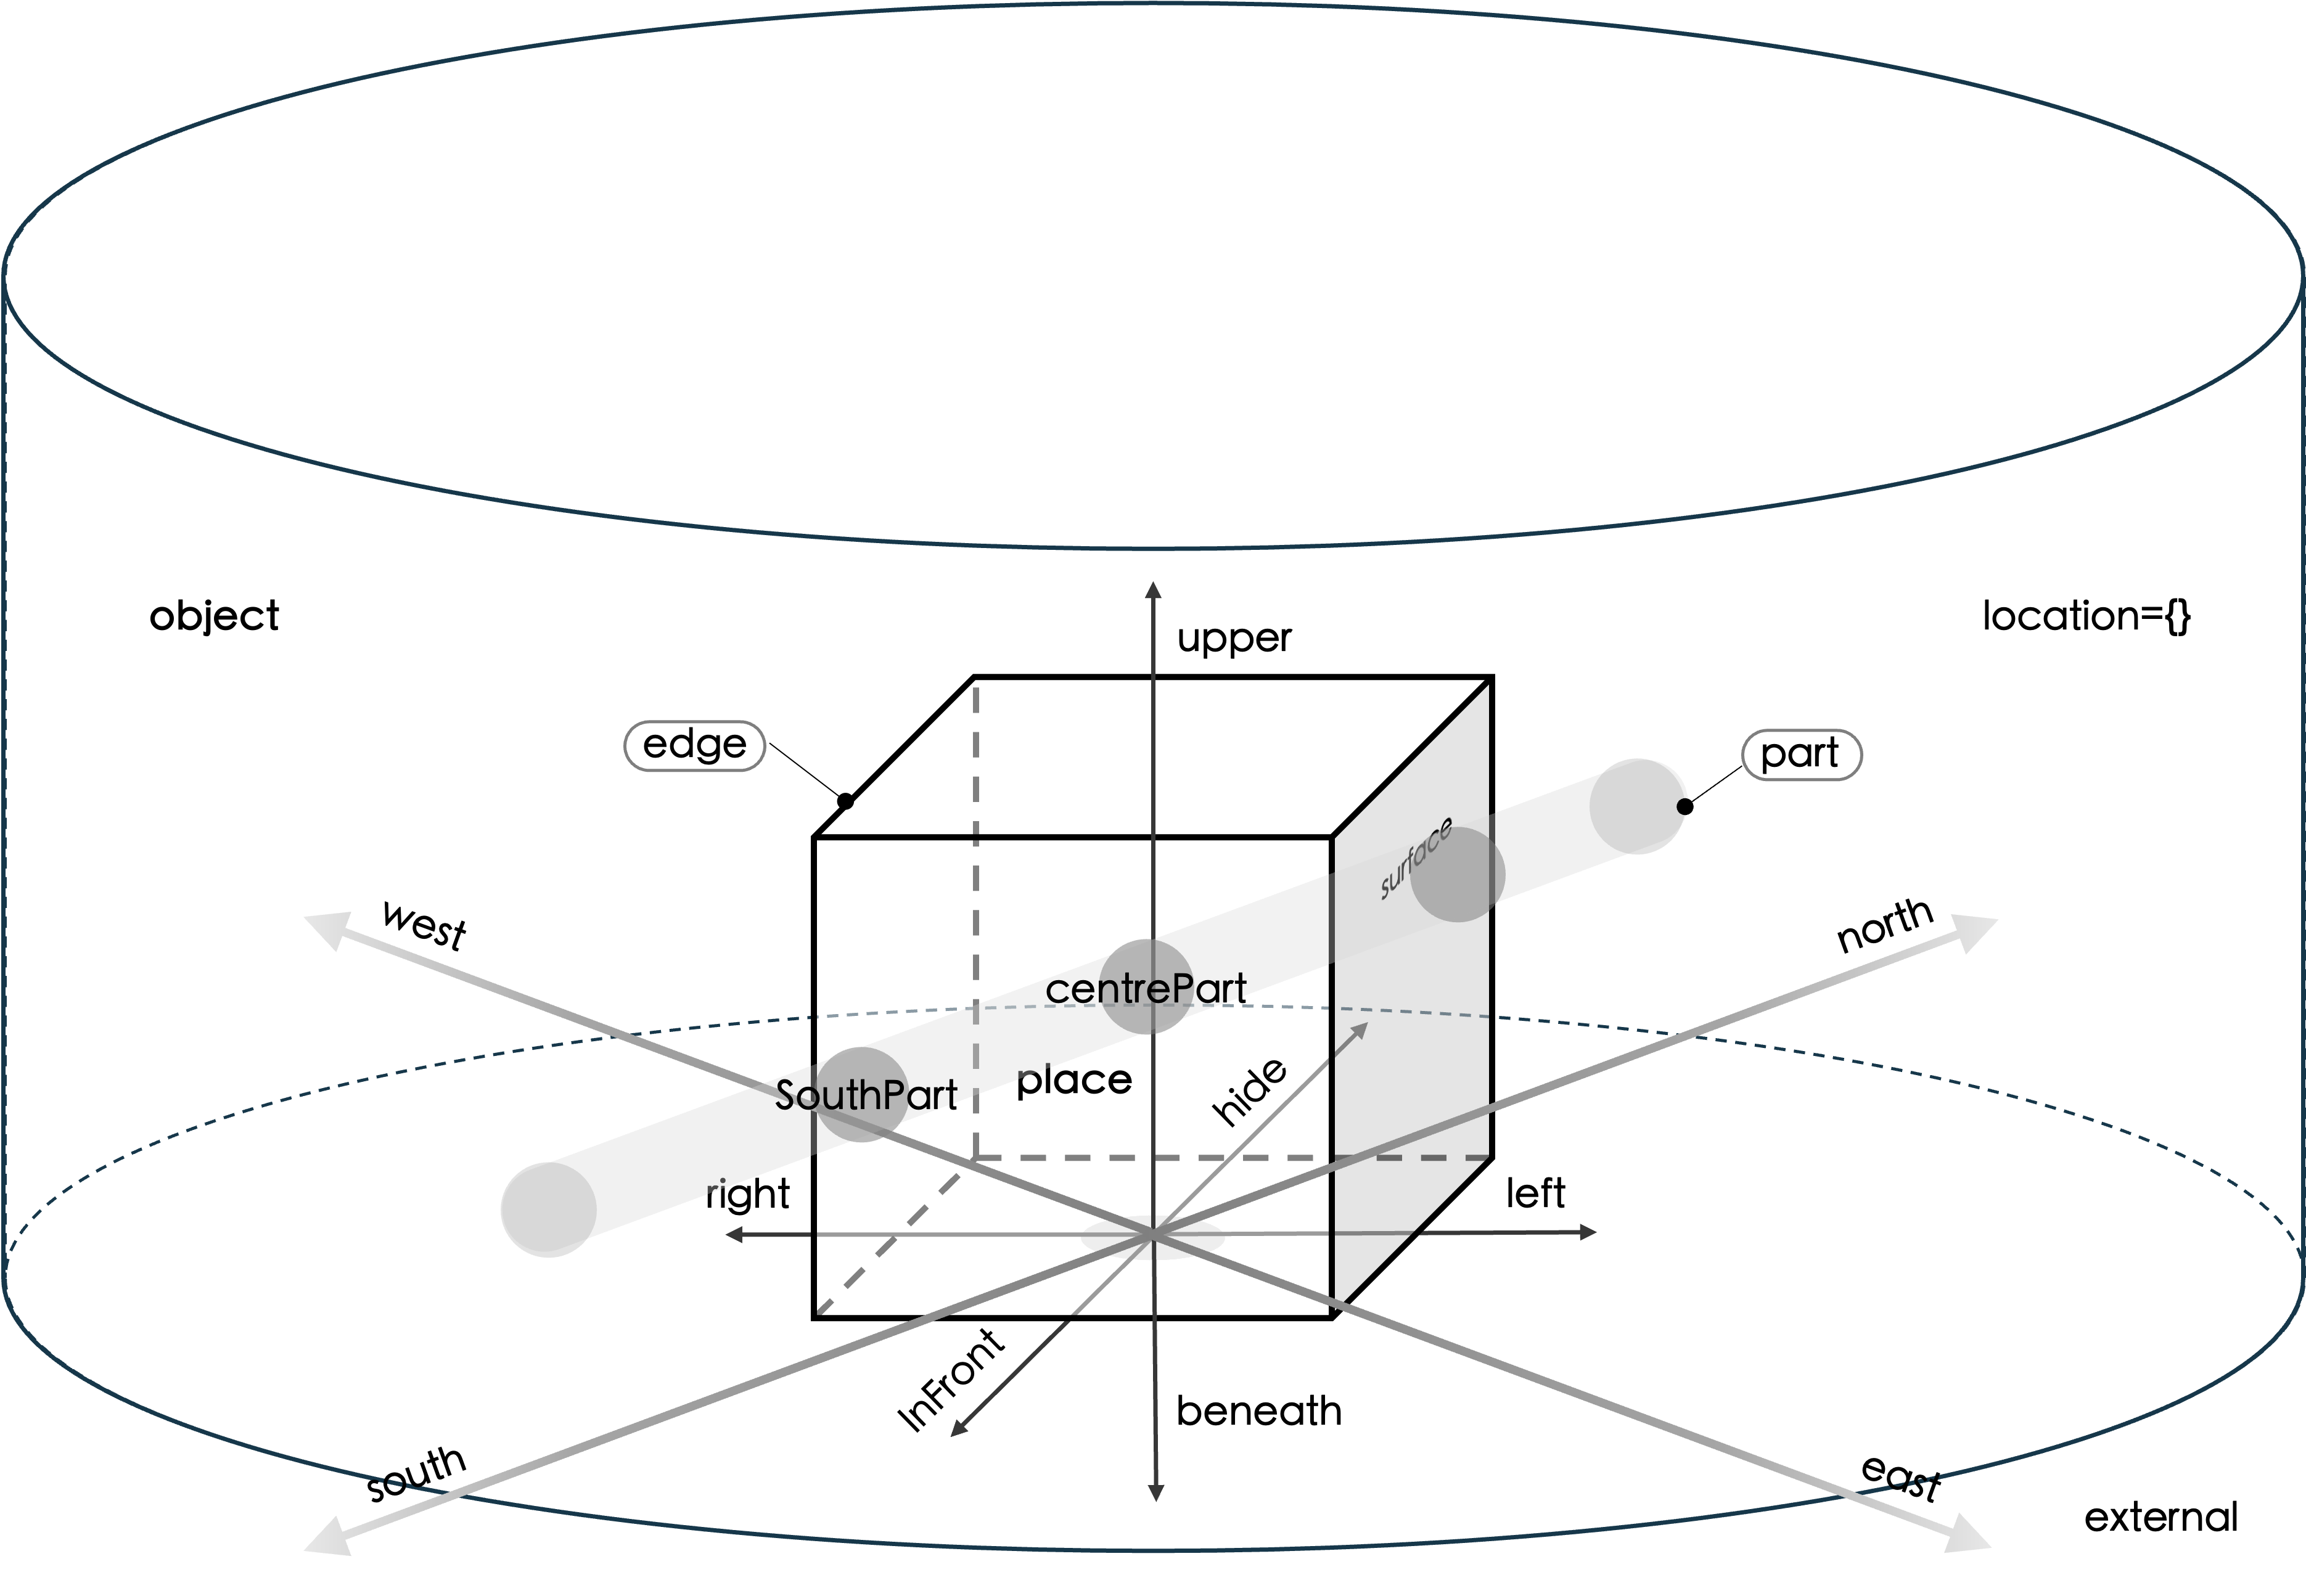
\includegraphics[width = \textwidth]{figures/spatialpreposition.png}
\caption{空間介詞與方位詞之語意圖(改自\citet{RN45})}
\label{fig:spatialpreposition}
\end{figure}

{\footnotesize
\renewcommand{\arraystretch}{0.8}
\begin{longtable}{
  >{\centering\arraybackslash}m{1cm} % 第一欄寬 1cm,水平置中且垂直置中
  >{\centering\arraybackslash}m{1cm} % 第二欄
  >{\arraybackslash}m{6cm}            % 第三欄,垂直置中,水平靠左
  >{\arraybackslash}m{3cm}            % 第四欄
  >{\arraybackslash}m{2cm}            % 第五欄
}
\caption{空間介詞與方位詞列表} \label{tab:wordList} \\
\toprule
詞彙 & 詞性 & E-HowNet表達式 & 詞意 & 空間介詞/方位詞 \\
\toprule
\endfirsthead
\toprule
詞彙 & 詞性 & E-HowNet表達式 & 詞意 & 空間介詞/方位詞 \\
\toprule
\endhead
\bottomrule
\endlastfoot
在 & P & location=\{\} & in, at, on, etc. & at(在) \\ \hline
外 & Ncda & \{external|外\} & outside & out(外) \\ \hline
中 & Ncdb & \{internal|內\} & inside & in(裡) \\ \hline
上 & Ncda & \{upper|上\} & on, above & on, above \\ \hline
下 & Ncda & \{beneath|下\} & below, under, underneath & down, below \\ \hline
前 & Ncda & \{InFront|前\} & front & front \\ \hline
後 & Ncda & \{hide|後\} & rear, back, behind & behind \\ \hline
左 & Ncda & \{left|左\} & left side, east, the Left & left \\ \hline
右 & Ncda & \{right|右\} & right side, the Right, west & right \\ \hline
北 & Ncda & \{north|北\} & north & North \\ \hline
西 & Ncda & \{west|西\} & west & West \\ \hline
東 & Ncda & \{east|東\} & east & East \\ \hline
南 & Ncda & \{south|南\} & south & South \\ \hline
面 & Ncda & \{surface|表層\} & surface, top, face & side, face \\ \hline
邊 & Ncda & \{edge(\{place|地方\})\} & border, boundary & side \\ \hline
上部 & Ncdb & \{TopPart|頂端\} & upper part, volume 1 & part \\ \hline
頂部 & Ncdb & \{TopPart|頂端\} & top & \\ \hline
底部 & Ncdb & \{BasePart|底部\} & bottom & \\ \hline
末端 & Ncdb & \{EndPart|尾部\} & tip, end & \\ \hline
中北部 & Ncdb & \{NorthPart(\{CentrePart(\{place|地方\})\})\} & midnorth & \\ \hline
中南部 & Ncdb & \{SouthPart(\{CentrePart(\{place|地方\})\})\} & middle and southern part & \\ \hline
中西部 & Ncdb & \{WestPart(\{CentrePart(\{place|地方\})\})\} & midwest & \\ \hline
中部 & Ncdb & \{CentrePart(\{place|地方\})\} & midland, central section & \\ \hline
北部 & Ncdb & \{NorthPart(\{place|地方\})\} & northern part & \\ \hline
南部 & Ncdb & \{SouthPart(\{place|地方\})\} & southern part & \\ \hline
東北部 & Ncdb & \{NorthPart(\{EastPart(\{place|地方\})\})\} & northeast & \\ \hline
東南部 & Ncdb & \{SouthPart(\{EastPart(\{place|地方\})\})\} & southeast & \\ \hline
東部 & Ncdb & \{EastPart(\{place|地方\})\} & east & \\ \hline
西北部 & Ncdb & \{NorthPart(\{WestPart(\{place|地方\})\})\} & northwest & \\ \hline
西南部 & Ncdb & \{SouthPart(\{WestPart(\{place|地方\})\})\} & southwest & \\ \hline
西部 & Ncdb & \{WestPart(\{place|地方\})\} & western part & \\ \hline
上游 & Ncb & \{TopPart(\{河|river\})\} & upper reaches of river & \\ \hline
中下游 & Ncb & \{union(\{CentrePart(\{河|river\})\},\{EndPart(\{河|river\})\})\} & middle and lower reaches & \\ \hline
中游 & Ncb & \{CentrePart(\{河|river\})\} & middle reaches & \\ \hline
下游 & Ncb & \{EndPart(\{河|river\})\} & lower reaches & \\ \hline
左端 & Ncdb & \{EndPart(\{object|物體\}):position=\{left|左\}\} & left end & \\ \hline
右端 & Ncdb & \{EndPart(\{object|物體\}):position=\{right|右\}\} & right end & \\ \hline
北端 & Ncdb & \{EndPart(\{object|物體\}):position=\{north|北\}\} & northern end & \\ \hline
西端 & Ncdb & \{EndPart(\{object|物體\}):position=\{west|西\}\} & west end & \\ \hline
南端 & Ncdb & \{EndPart(\{object|物體\}):position=\{south|南\}\} & south end & \\ \hline
東北端 & Ncdb & \{EndPart(\{place|地方\}):position=\{north(\{east|東\})\}\} & northeast end & \\ \hline
東南端 & Ncdb & \{EndPart(\{place|地方\}):position=\{south(\{east|東\})\}\} & southeast end & \\ \hline
西北端 & Ncdb & \{EndPart(\{place|地方\}):position=\{west(\{north|北\})\}\} & northwest end & \\ \hline
西南端 & Ncdb & \{EndPart(\{place|地方\}):position=\{west(\{south|南\})\}\} & southwest end & \\ \hline
方 & Ncda & \{place|地方\} & direction, place, region & direction, axis \\ \hline
東方 & Ncdb & \{east|東\} & eastern & \\ \hline
東邊 & Ncdb & \{east|東\} & east & \\ \hline
東西方 & Ncdb & \{union(\{east|東\},\{west|西\})\} & east and west & \\ \hline
西方 & Ncdb & \{west|西\} & western & \\ \hline
西邊 & Ncdb & \{west|西\} & west side & \\ \hline
北方 & Ncdb & \{north|北\} & north, northern area & \\ \hline
東北方 & Ncdb & \{north(\{east(\{object|物體\})\})\} & northeastward & \\ \hline
南方 & Ncdb & \{south|南\} & southern & \\ \hline
東南方 & Ncdb & \{south(\{east(\{object|物體\})\})\} & southeastward & \\ \hline
右方 & Ncdb & \{right|右\} & the right side & \\ \hline
左方 & Ncdb & \{left|左\} & the left side & \\ \hline
上方 & Ncdb & \{upper|上\} & above, on top & \\ \hline
下方 & Ncdb & \{beneath|下\} & below, lower & \\ \hline
前方 & Ncdb & \{InFront|前\} & ahead, front direction & \\
\end{longtable}
}

綜合上述討論,圖10顯示本研究發展之位置描述知識本體的空間介詞與方位詞及其概念串接至上層知識本體的結構。詳細來說,在\textit{locd:SpatialConcpet} (空間概念)下記錄\textit{locd:SpatialRelationship} (空間關係),依據E-HowNet之定義可再進一步細分為三個主要與位置表達相關的類別,分別為\textit{ehn:LocationFunction} (位置函數)、\textit{ehn:DistanceValue}和\textit{ehn:AlterLocation} (變空間位置)。

與空間概念關係相對的,在\textit{locd:LocationDescription}相關的兩個類別\textit{locd:SpatialPreposition}和\textit{locd:Localizer}會記錄E-HowNet的詞彙資訊,又以E-HowNet中對於詞意作為細分,對應著\textit{locd: SpatialRelationship}的各個類別組成,例如:\textit{ehn:NortheastPartLocaliser} (東北部)對應著\textit{ehn:NorthPart}和\textit{ehn:EastPart},又\textit{ehn:東北部}會作為\textit{ehn: NortheastPartLocaliser}當中的一個實例。如此一來,表 7之清單會以知識本體形式記錄下,以供後續語意查詢與語意規則推論機制。

\section{空間認知三階段規則}

為了實現位置描述的自動化從空間資料中產生,本研究建構空間認知三階段規則。這些規則能夠係透過位置描述知識本體橋接O-SLD三層式框架的前後兩層,進而支持情境感知的語意推論與產生語意式的位置描述。在本研究的建構之規則知識,以語意網規則語言(semantic web rule language, SWRL)的方式紀錄,並分為:情境影響參考物、資料層到語意層和語意層到自然語言層三階段,\ref{tab:ruleDemo}為簡單範例顯示這三個階段如何構成一套可擴充且具備語意解釋能力的推論框架,為後續位置詞彙的生成提供知識基礎,本節將詳細說明三個階段的設計準則與內容。

\lstset{basicstyle=\ttfamily\scriptsize, breaklines=true}
\begin{table}[htbp]
\centering
\caption{規則推論階段範例}
\label{tab:ruleDemo}
\begin{adjustbox}{max width=\textwidth}
\renewcommand{\arraystretch}{1.4}
\begin{tabular}{
>{\centering\arraybackslash}m{1cm} >{\centering\arraybackslash}m{2.5cm} >{\centering\arraybackslash}m{10cm} >{\centering\arraybackslash}m{2.5cm}}
\toprule
項次 & 階段 & 規則簡單範例 & 敘述 \\
\toprule
1 & 情境影響參考物選擇 & \texttt{AnyContext(?ctx)\^{}AnyType(?ref)\^{}SpatialOperation(?rel) -> GroundFeature(?ref)\^{}hasGroundFeature(?rel, ?ref)} & 任一情境下選擇任一物件類型作為參考物 \\
\hline
2 & 資料層到語意層 & \texttt{AnyContext(?ctx)\^{}Distance(?rel)\^{}hasDistance(?rel, ?d)\^{}swrlb:lessThan(?d, 300) -> Near(?rel)} & 在任一情境中少於300被視爲「近」 \\
\hline
3 & 語意層到自然語言層 & \texttt{WorsSense(?s)\^{}Word(?w) -> hasSpatialPreposition(?w)/hasLocaliser(?w)} & 詞意詞彙對照 \\
\hline
\bottomrule
\end{tabular}
\end{adjustbox}
\end{table}

\subsection{情境影響參考物選擇}

第一階段聚焦於情境如何影響參考物的選擇,在空間資料中,參考物類別繁多,然而在特定情境下,並非所有參考物皆具備語意位置描述的價值。因此,本階段的目的為根據情境,自動篩選出在該情境下具參考價值的空間物件類別,並賦予其語意角色,以利後續的語言生成與推理。舉例而言,在交通情境中,偏好識別道路及道路相關的空間物件,而忽略如海域、山脈或水體等地物。

本研究在位置描述知識本體中定義了情境(如交通和災防告警)與Feature類型(如建物和山脈等)都被記錄並形式化於知識本體中,在此階段的推論中,將透過SWRL規則對不同物件給定「參考物(\textit{locd:GroundFeature})」角色,以支持後續的推論中連結到參考物及其性質。例如:

\begin{lstlisting}[language=Prolog, basicstyle=\ttfamily, xleftmargin=2em]
Traffic(?ctx)^Road(?ref)^SpatialOperation(?rel) 
->GroundFeature(?ref)^hasGroundFeature(?rel, ?ref)
\end{lstlisting}

此規則表示,在Traffic (交通情境)下,Road (道路)視為GroundFeature (參考物件)這個角色。
除情境規則外,亦可擴充不依賴特定情境或物件之通用規則,例如:

\begin{lstlisting}[language=Prolog, basicstyle=\ttfamily, xleftmargin=2em]
GeneralContext(?ctx)^Feature(?ref)^SpatialOpeartion(?rel)
->GroundFeature(?ref)^hasGroundFeature(?rel, ?ref)
\end{lstlisting}

此規則表示,只要是Feature (圖徵)即是GroundFeature (參考物件)這個角色。

\subsection{資料層到語意層}

第二階段聚焦於空間語意的推論,此階段的目的是將空間物件與各類空間操作合理轉化為語意上的空間關係,進而為後續產生位置描述提供基礎。舉例而言,對於語意上的空間關係「Upper」,若參考物為「建物」與「公園」,在人類解讀上可能會產生不同的語意。若參考物改為「建物」,「Upper」則可能指目標物在建物頂樓上方,且這樣的空間關係是具有普遍性,對於建物大多能達成。然而,若「公園」為參考物,日常鮮少會描述自己位於公園「上」,因此若無考量參考物之語意,可能會造成不合理的推論結果。

在此階段中,透過 SWRL 規則對不同類型的Feature及其語意進行推論,以確保語意層的合理性與準確性,本研究將設計一組關鍵空間操作通用規則集,包括「Intersects」和「Touches」等空間操作,例如:

\begin{lstlisting}[language=Prolog, basicstyle=\ttfamily, xleftmargin=2em]
Within(?rel)^FigureFeature(?tar)^hasFigureFeature(?rel, ?tar)
^GroundFeature(?ref)^hasGroundFeature(?rel, ?ref)
->OnSite(?rel)
\end{lstlisting}

此規則表示,在目標物與參考物存在GIS空間操作「Within」,則視為語意上的空間關係「OnSite」。
此外,根據特性考慮結合Feature性質(主要為幾何類型、類別和其他性質),以達成無法直接從空間操作中描述的語意空間關係,例如:

\begin{lstlisting}[language=Prolog, basicstyle=\ttfamily, xleftmargin=2em]
Within(?rel)^FigureFeature(?tar)^hasFigureFeature(?rel, ?tar)
^GroundFeature(?ref)^hasGroundFeature(?rel, ?ref)
^hasQuality(?ref, ?form)
^StyleandForm(?form)^qualityValue(?form, “elevated”)
->Upper(?rel)
\end{lstlisting}

此規則表示,在目標物與參考物存在GIS空間操作「Within」,且當參考物存在StyleandForm(型態)為「elevated(帶有高程)」時,則視為語意上的空間關係「Upper」,以此來建構具語意合理性的推論。

綜述而言,該階段透過知識本體與SWRL規則的結合,確保空間語意推論結果的合理性,既能反映Feature之間的真實關係,又能符合人類語意表達的邏輯與常識。

\subsection{語意層到自然語言層}

第三階段的重點是將語意層的推論結果轉化為自然語言描述,以實踐產生自然語言形式的位置描述。本階段的目標是產生能夠符合人類閱讀與解釋習慣的自然語言描述,同時保持語意的一致性與精確性。為提升自然語言生成的靈活性,本研究將採用基於模板(template-based)的生成方法,結合情境化規則進行描述細化。在語意轉化過程中,將結合 SWRL 推論結果與自然語言生成(natural language generation, NLG)技術,逐步將知識本體中的語意規則映射至語意結構,例如:

\begin{lstlisting}[language=Prolog, basicstyle=\ttfamily, xleftmargin=2em]
OnSite(?rel)^LocationDescription(?locad)
^symbolize(?rel, ?locad)^AtSpatialPreposition(?word)
->hasSpatialPreposition(?locad, ?word)
\end{lstlisting}

此規則表示,當存在空間關係為「OnSite」時,會推得出 AtSpatialPreposition (「在」的空間介詞),因此 LocationDescription (位置描述)可獲得空間介詞為「在」。

\section{情境分析}

在近幾年對於防救災的重視與體制發展下,「如何將以坐標記錄的圖徵位置轉化為人類可理解的語言描述」已成為災害傳達與決策的重要課題。本研究聚焦兩個諸如防救災等需及時提供文字式位置描述傳達給民眾或有關單位的應用情境,分別為:交通情境和災防告警,以探討語意式位置描述在實務中的角色和挑戰。

首先,在交通情境中,如警察廣播電台所建置的即時路況系統,即爲一種群眾參與的語意式位置回報機制。透過設有路況服務專線,接受民眾提供的路況,提供了事故、交通壅塞和道路施工等主題之路況描述(警察廣播電臺, 2021)。除了路況說明,也包含了自然語言文字式的空間位置與地點描述及坐標資訊,當中的位置描述以自然語言傳達可使民眾更快速且直觀理解位置所在,而不需額外讀地圖和理解圖徵及圖幅方位等地圖意涵,提供位置理解速度與傳播效率。

其次,在災防告警情境中,常見例如災防告警細胞廣播訊息係透過經緯度記錄之空間幾何決定其發布範圍,即手機使用在該範圍內基地台的民眾會收到細胞廣播,為使民眾快速了解發生地點或影響地點,在訊息中會附帶上位置描述(張子瑩等人., 2016)。例如,在地震速報一類中會放上「東北海域」等描述,在大雷雨訊息中會以「您所在地」提醒民眾位於何處。其中,「東北海域」這一描述是基於與台灣本島的空間方位關係而產生,在目前的機制下除事先建構地名辭典,否則無法產生。

上述兩個案例凸顯語意式位置描述在防救災資訊傳遞與空間理解中的實用性與必要性,同時也顯示出現行機制在語意生成與對應規則上的不足之處,為本研究提供了具體的問題場域與應用動機。

圖 \ref{fig:context_steps} 顯示情境分析步驟,分別為LocD知識本體擴展、情境關聯之規則定義和樣板設計,本節將詳細說明兩個情境中的三個工作流。

\begin{figure}[!htbp]
\centering

\includegraphics[width = \textwidth]{figures/conext_steps.png}
\caption{情境分析流程}
\label{fig:context_steps}
\end{figure}

\subsection{交通情境}

\subsubsection{LocD知識本體擴展}

在交通相關的情境中,知識本體需表示的不僅是道路的類型,還包括道路段、交叉路口與附屬設施。為了回應真實世界情境與領域語意的需求,本研究個案擴充了LocD知識本體,納入更細緻的道路網系統分類,這在交通情境中扮演關鍵角色。

知識本體中空間物件的「類別」係依據內政部發布的《地形圖資分類架構》,為了彌合通用分類與情境中領域專屬類型間的落差,本研究引入交通部發布之《交通網路基本資料標準(第一版)》,該標準定義了臺灣交通系統的結構。此分類已整合至LocD知識本體作為其子結構,如圖六所示。

\subsubsection{情境關聯之規則定義}

這些交通情境與對應的參考物件也進一步連結至第 3.3 節所述的具情境感知之推論規則,使系統在語意推理過程中能動態決定符合情境的參考物件。基於警察廣播電台提供的 2,000 筆即時交通通報資料,本研究使用實體命名辨識(named entity recognition, NER)技術,將原始的非結構化資料轉換為結構化格式,並進行語意標註(semantic annotation),藉此識別在交通語境中常被使用的參考物件類型。

\begin{lstlisting}[language=Prolog, basicstyle=\ttfamily, xleftmargin=2em]
SpatialOperation(?rel)^hasContext(?rel, ?ctx)^Traffic(?ctx)
^Feature(?f)^hasFeature(?rel, ?f)^hasQuality(?f, ?type)
^UndergroundUrbanRoad(?type)^FigureFeature(?ff) 
->hasFigureFeature(?rel, ?ff)
^GroundFeature(?f)^hasGroundFeature(?rel, ?f)
\end{lstlisting}

\subsubsection{樣板設計}

\subsection{災防告警情境}

\subsubsection{LocD知識本體擴展}

\subsubsection{情境關聯之規則定義}

\subsubsection{樣板設計}


\section{評估方法}
本研究採用SPICE(Semantic Propositional Image Caption Evaluation)作為評估指標\citep{RN29},以衡量機制產生之候選描述與參考描述之間的語意對齊程度。相較於傳統以字串層級為主的評估指標(如BLEU和ROUGE),或近年來基於大型語言模型之語意層級評估指標(如BERTScore),SPICE 能更準確反映語句的語意結構及實體匹配,適合本研究所關注之語意式位置描述任務。

SPICE主要以F1 score作為核心指標,綜合考量語意單元的準確率(Precision)與召回率(Recall)。語意單元係指候選與參考描述文字透過語意場景圖(semantic scene graphs)分析後所產生的三元組(triple)集合,其形式為「(object)」、「(object, attribute)」、「(object, relation, object)」三者。其中,準確率表示機制產生的語意單元中,有多少與參考描述一致;召回率則反映參考描述中的語意單元,有多少被機制成功捕捉;F1 分數則為兩者的調和平均,用以綜合評估語意重合程度。其數學定義如下(式 \ref{eq:spice_p} 、 \ref{eq:spice_r} 和 \ref{eq:spice_f1} ),其中準確率為$P$、召回率為$R$,$c$為候選文字、$S$為參考文字、$T(G(c))$為候選三元組集合、$T(G(S))$為參考三元組集合,而$\otimes$意味集合匹配與否。

\begin{equation}
\label{eq:spice_p}
P(c,S) = \frac{\left| T(G(c)) \otimes T(G(S)) \right|}{\left| T(G(c)) \right|}
\end{equation}

\begin{equation}
\label{eq:spice_r}
R(c,S) = \frac{\left| T(G(c)) \otimes T(G(S)) \right|}{\left| T(G(S)) \right|}
\end{equation}

\begin{equation}
\label{eq:spice_f1}
SPICE(c,S) = F_1(c,S) = \frac{2 \times P(c,S) \times R(c,S)}{P(c,S) + R(c,S)}
\end{equation}

在本研究之任務中,語意單元統一定義為「(空間介詞, 地點名稱, 方位詞)」之三元組形式,例如:位置描述「在中山高速公路上」將被轉換為「(在, 中山高速公路, 上)」的三元組。為確保評估準確性與參考資料的一致性,本研究之參考描述之真值(ground truth)經由個案分析後人工標記產生,經人工語意理解後轉換為三元組形式。

此外,為處理同地異名和同義詞情況,本研究建立了地理實體對應辭典,以統一地點名稱的語意指涉,例如:「中山高速公路」、「國道一號」或「國1」等應視為指涉相同地理實體。同時,針對空間介詞及方位詞的匹配操作,本研究採用E-HowNet中文詞庫作為語意相似度的判斷依據,例如:「位於」和「在」在E-HowNet上會視為是同義詞。基於SPICE指標結合地理辭典與中文詞庫,本研究提升了三元組匹配的語意靈敏度與評估準確性。



% !TeX root = ../main.tex

\chapter{基於知識本體之位置描述的網路網路地理資訊系統應用整合}

本研究開發了一個基於知識本體之語意式位置描述的網際網路地理資訊系統(Web Geographic Information System, WebGIS)應用,其核心架構整合知識本體、SWRL規則推論、GIS和網頁,以實現語意式位置描述的產生與應用(參見圖 11)。

本研究的系統架構包含兩大資源層,分別為「GIS資源層」和「語意資源層」。GIS資源層負責Feature記錄與空間操作,本研究採用PostgreSQL空間資料庫進行儲存,以提供API介接,並支援應用開發;語意資源層涵蓋位置描述知識本體與SWRL規則集,用以推導位置語意資訊,確保語意式位置描述的完整性與合理性。本研究在知識本體的建構過程中,採用OWL (Web Ontology Language)作為知識表示工具,並利用Protégé進行編輯,以確保語意結構的完整性與標準化。此外,本研究設計了一套基於SWRL的推論規則集,該規則可用於模擬空間物件的關係推理與語意合理性檢驗,當中包含兩階段的推論(即空間關係推論和詞意推論)。

本研究的WebGIS應用採用API介接模式,使用者發送請求並接收回應,其中:請求為任一Feature,回應則為文字式的位置描述。程式執行流程概述如下:第一,空間關係查詢與紀錄,即透過輸入Feature和存在於資料庫中的參考空間物件。本研究開發API提供空間關係查詢與記錄,開發環境選用為Node.js,並結合基於JavaScript的空間操作函式庫Turf.js進行方便且快速的空間關係查詢。而後,進行語意推論與位置描述生成。根據前述所獲得的空間操作關係組,會進一步將內容映射至知識本體,並透過SWRL規則進行推論。該一過程透過Python的Owlready2套件進行知識本體的載入、推理與規則驗證,以實踐自動化推理功能,當中的推論器為Pellet reasoner。

本研究最終將發展一組API及WebGIS應用,以坐標產生位置描述的逆向地理編碼機制,提升地理資訊在多元領域的應用價值。系統主要包含兩項功能:其一,使用者可透過API存取服務,將現有的歷史資料中附有坐標的空間資訊自動轉換為文字化的位置描述,滿足大規模資料處理需求;另一,透過WebGIS介面,使用者可以即時繪製空間範圍,並獲取範圍內對應的位置描述結果。該功能提供即時性且直覺的使用體驗,特別適用於探索性分析與小範圍資料需求。此外,為促進研究持續增進,在介面上將設計回饋機制以蒐集結果準確性及適宜性的評估資料,進一步作為未來改良位置描述編碼機制之參考基礎。

% !TeX root = ../main.tex

\chapter{案例研究}

本章說明位置描述知識本體和O-SLD框架的可行性實踐。本研究選擇警察廣播電台即時路況與災防告警細胞廣播訊息作為案例作為分析對象,以探討其對應情境中的位置描述。為此,首先擴展了道路和災防領域的位置語意之知識本體,以提升語意標註的完整性和適用性。接著,透過實驗結果和實體匹配之評估,驗證本研究方法在這兩個領域中產生位置描述的有效性。本節內容詳細如下:在4.1節中,介紹了實驗區的選擇與圖資;在4.2節說明案例動機、知識本體建構結果,以及語意式位置描述產出;在4.3節呈現案例評估之結果,並討論本研究提出方法適用性。

\section{實驗區及圖資介紹}

本研究選定臺灣地區十萬分之一索引圖中的「9723」圖框範圍(參見圖 12),其介於北緯25度到25.5度和東經121.5度到122度之間,主要考量以下因素:首先,空間物件的多樣性,「9723」區域涵蓋都市、鄉村、山地及海洋水體等多種地理環境,有助於測試位置描述本體在不同空間物件類型下的適用性與語意描述能力,確保模型能夠應對各類地理情境。其次,區域的代表性,「9723」圖框範圍內包含臺灣首都臺北市,擁有密集的道路網絡與豐富的人為設施,使其成為語意式位置描述的理想測試案例,進一步提升研究成果的適用性與擴展性。第三,災害應變與道路通報應用的需求,該區域具有豐富的災害示警歷史記錄,且包含各層級的道路路網,適合作為災害示警與道路分析的應用情境,驗證本研究方法在實際應用中的可行性。最後,空間尺度適中,「9723」圖框範圍既不過於廣泛,以致運算與分析負擔過大,亦不過於狹小,以免影響研究結果的普適性。適當的空間尺度有助於在合理的資源限制下,進行有效的語意標註與分析。

圖資使用為110年瑞竣科技電子地圖集,其圖層清單包含:道路中心線、鐵路、捷運、河流、縣市界、基礎地標、山峰等28類圖層(參見表 9)。

\section{研究結果}

\section{評估與討論}
% !TeX root = ../main.tex

\chapter{結論與未來展望}

本研究不僅拓展了逆向地理編碼的新視角,也在交通與災防告警的情境中展現了具體的實務可能和貢獻。在研究方法上,本研究所提出之 O-SLD 位置描述生成機制具有以下三項主要特色:第一,可接受點、線、面等各種形狀的空間物件作為輸入;第二,可彈性結合多個空間參考物;第三,可整合知識本體與 SWRL 規則進行語意限制。這些特性使得產生之自然語言式位置描述具備更豐富的結構與資訊內容,從空間關係與尺度觀點更貼近人類理解的位置,實現將GIS坐標紀錄之物件轉譯為具語意更易溝通及閱讀的位置描述文字。

在實務應用層面,系統已於災防告警與交通案例中展現效益,能根據情境及空間尺度,自動化產生合適的位置描述,提供更貼近使用者認知的語句建議,進而應用於基於位置服務之地點描述、警示訊息自動生成與地圖輔助描述等,例如:災防單位結合本研究提出 O-SLD 機制,僅需輸入 GeoJSON,即可快速獲得多組語意化位置描述建議,提升作業效率與溝通清晰度。

未來研究可延伸本研究之架構,發展更多樣化的語意位置描述類型,並與特定領域情境結合,擴展知識本體與語意規則於自然語言地理描述的應用層面,進一步提升語意標註的廣度與深度。本研究亦存在若干限制。首先,位置描述的精確性仍依賴知識本體的完備程度與參考物的給予,當參考物資料不完整時,本研究機制無法從無資料中產生最理想的描述。例如,目前知識本體及空間物件僅考量二維GIS中的表達,涉及三維的地物則無法處理,仍待未來研究進一步結合本研究發展之位置描述知識本體擴充。其次,本研究結合知識本體建構出人如何理解位置的理論框架,然實際語意推論能力受制於情境及使用者的多元性,未來研究可透過經驗研究方式待量化人的空間感知與語句偏好,進一步提升位置描述的語意精準度和使用者體驗。


% 參考文獻
% References
\refmatter
% \printbibliography                   % <- 你可以直接把中英的參考文獻混再一起

% \printbibheading                       % <- 或者分中文與英文兩部分,但記得在reference.bib中要加入keyword
% \section*{一、英文部分}
% \printbibliography[keyword = {english}, heading = none]
% \section*{二、中文部分}
% \printbibliography[keyword = {chinese}, heading = none]

% 附錄
% Appendices
% !TeX root = ../main.tex

\appendix{A}{Result and Evaluation}
\section{Result}

\begin{table}[htbp]
\centering
\caption{標記之真值}
\label{tab:groundTrue}
\begin{adjustbox}{max width=\textwidth}
\renewcommand{\arraystretch}{1.4}
\begin{tabular}{>{\centering\arraybackslash}m{1cm} >{\centering\arraybackslash}m{4cm} >{\centering\arraybackslash}m{4cm} >{\centering\arraybackslash}m{4cm} >{\centering\arraybackslash}m{4cm}}
\toprule
項次 & 圖面/經緯度坐標 & 本研究機制 & 人工撰寫 & GPT-4o \\ 
\toprule
1-1 & & 中山高速公路12.1公里附近(汐止系統交流道)& 北上在12公里到7公里之間.汐止系統前~五堵.內線. & 位於新北市汐止區,鄰近台北101東北約10公里,靠近國道一號汐止交流道,附近有基隆河,屬於住宅區。 \\ \hline
1-2 & & 新北市瑞芳區瑞濱路(龍潭堵隧道) & 西行在18.4公里到17.3公里之間.龍潭堵隧道 & 位於新北市瑞芳區,靠近九份老街東南約300公尺,鄰近基山街和輔仁路交會處,接近基隆河岸,屬於觀光區。 \\ \hline
1-3 & & 在臺北市大安區和平東路二段118巷2弄(科技部附近) & 和平東路二段118巷2弄16號 & 位於台北市大安區,鄰近台北101東北約1公里,靠近信義路四段與基隆路交叉口,臨近大安森林公園,屬於商業區。 \\ \hline
1-4 & & 在臺北市大同區民權西路路口(捷運民權西路站附近)  & 承德路二段+民權西路口 & 位於台北市中正區,靠近台北車站東南約300公尺,鄰近忠孝西路與館前路交會處,周圍為商業區中心。 \\ \hline
1-5 & & 在臺北市大安區建國南北快速道路上(忠孝東路三段上方) & 建高往北.忠孝東路上方 & 位於台北市大安區,鄰近台北101東北約1公里,靠近信義路和復興南路交會處,接近大安森林公園,屬於商業區。 \\ \hline
1-6 & & 在台北大橋 & 台北橋往台北 & 位於台北市信義區,鄰近台北101東北約300公尺,靠近信義路五段與松智路交會處,臨近基隆河岸,屬於商業區中心。 \\ \hline
2-1 & & & & \\ \hline
2-2 & & & & \\ \hline
2-3 & & & & \\ \hline
3-1 & & & & \\ \hline
3-2 & & & & \\ \hline
3-3 & & & & \\ \hline
4-1 & & & & \\ \hline
4-2 & & & & \\ \hline
4-3 & & & & \\ \hline
5-1 & & & & \\ \hline
5-2 & & & & \\ \hline
5-3 & & & & \\
\bottomrule
\end{tabular}
\end{adjustbox}
\end{table}

\section{Evaluation}

\begin{table}[htbp]
\centering
\caption{標記之真值}
\label{tab:groundTrue}
\begin{adjustbox}{max width=\textwidth}
\renewcommand{\arraystretch}{1.4}
\begin{tabular}{>{\centering\arraybackslash}m{1cm} >{\centering\arraybackslash}m{16cm} }
\toprule
項次 & 內容 \\
\toprule
1-1 & ("在", "新北市", None), (None, "瑞芳區", None), (None, "萬瑞快速道路", "上"), ("西行", None, None), (None, "瑞濱端", None), (None, "龍潭堵隧道", "內") \\
\hline
1-2 & (None, None, "北上"), ("在", "中山高速公路", "上"), (None, "10.5公里", "處"), (None, "汐止交流道", None) \\
\hline
1-3 & ("在", "臺北市",  None), (None, "大安區", None), (None, "和平東路二段118巷2弄", None), (None, "科技大樓", "後方"), (None, "科技部", "附近") \\
\hline
1-4 & ("在", "臺北市",  None), (None, "大同區", None), (None, "民權西路", "路口"), (None, "承德路二段", "路口"), (None, "捷運民權西路站", "附近"), (None, "台灣銀行", "附近"), (None, "台北大橋", "前") \\
\hline
1-5 & ("在", "臺北市",  None), (None, "大安區", None), (None, "建國南北快速道路", None), (None, "忠孝東路三段", "上方"), ("鄰近", "臺北科技大學", None) \\
\hline
1-6 & (None, "台北大橋",  None), ("往", "台北", None), ("在", "新店溪", "上") \\
\hline
2-1 & \\
\hline
2-2 & \\
\hline
2-3 & \\
\hline
3-1 & \\
\hline
3-2 & \\
\hline
3-3 & \\
\hline
4-1 & \\
\hline
4-2 & \\
\hline
4-3 & \\
\hline
5-1 & \\
\hline
5-2 & \\
\hline
5-3 & \\
\hline
\bottomrule
\end{tabular}
\end{adjustbox}
\end{table}

% % !TeX root = ../main.tex

\appendix{B}{Introduction}
\section{Introduction}
\section{Further Introduction}
               % <- 我先把原有的附錄先註解到了,你如果需要可以再重新加回

\end{document}